\documentclass[a4paper,12pt]{book}
\usepackage[utf8]{inputenc}
\usepackage{graphicx}
\usepackage{enumitem}
\usepackage{xcolor}
\usepackage{booktabs}
\usepackage{lscape}
\usepackage{ltablex}
\renewlist{itemize}{itemize}{20}

% initially, use dots for all levels
\setlist[itemize]{label=$\cdot$}

% customize the first 3 levels
\setlist[itemize,1]{label=\textbullet}
\setlist[itemize,2]{label=--}
\setlist[itemize,3]{label=*}

\begin{document}

\author{Standardisation Gang}
\title{Standards for subjectoriented specification of systems}
\date{August 2018}

\frontmatter
\maketitle
\tableofcontents

\mainmatter
% !TeX spellcheck = en_US

\chapter{Foundation}
Figures
To facilitate the understanding of the following sections we will introduce the philosophy of subject-orienting modeling which is based on the Parallel Activity Specification Scheme (PASS). Additional, we will give a short introduction to ontologies---especially the Web Ontology Language (OWL)---, and to Abstract State Machines (ASM) as underlying concepts of this standard document.

\section{Subject Orientation and PASS }
\label{SubjectOrient}

%\sidepar{Text in the sidebar}

In this section, we lay the ground for PASS as a language for describing processes in a subject-oriented way. This section is not a complete description of all PASS features, but it gives the first impression about subject-orientation and the specification language PASS. The detailed concepts are defined in the upcoming chapters.

The term subject has manifold meanings depending on the discipline. In philosophy, a subject is an observer and an object is a thing observed. In the grammar of many languages, the term subject has a slightly different meaning. "According to the traditional view, the subject is the doer of the action (actor) or the element that expresses what the sentence is about (topic)."~\cite{Keenan:1976aa}. In PASS the term subject corresponds to the doer of an action whereas in ontology description languages, like RDF (see section \ref{IntroOntology}), the term subject means the topic what the "sentence" is about.

\subsection{Subject-driven Business Processes}

Subjects represent the behavior of an active entity. A specification of a subject does not say anything about the technology used to execute the described behavior. This is different to other encapsulation approaches, such as multi-agent systems.

Subjects communicate with each other by exchanging messages. Messages have a name and a payload. The name should express the meaning of a message informally and the payloads are the data (business objects) transported. Internally, subjects execute local activities such as calculating a price, storing an address, etc.

A subject sends messages to other subjects, expects messages from other subjects, and executes internal actions. All these activities are done in sequences which are defined in a subject's behavior specification. Subject-oriented process specifications are always embedded in a context. A context is defined by the business organization and the technology by which a business process is executed.

Subject-oriented system development integrates established theories and concepts. It has been inspired by various process algebras (see e.g. [2], [3], [4]), by the basic structure of nearly all natural languages (Subject, Predicate, Object) and the systemic sociology developed by Niklas Luhmann (an introduction can be found in [5]). According to the organizational theory developed by Luhmann, the smallest organization consists of communication executed between at least two information processing entities [5]. The integrated concepts have been enhanced and adapted to organizational stakeholder requirements, such as providing a simple graphical notation, as detailed in the following sections.

\subsection{Subject Interaction and Behavior}

We introduce the basic concepts of process modeling in S-BPM using a simple order process. A customer sends an order to the order handling department of a supplier. He is going to receive an order confirmation and the ordered product by the shipment company. Figure \ref{fig:ordercomstructure} shows the communication structure of that process. The involved subjects and the messages they exchange can easily be grasped. 

%\strictpagecheck
\begin{figure}[htbp]
	\centering
	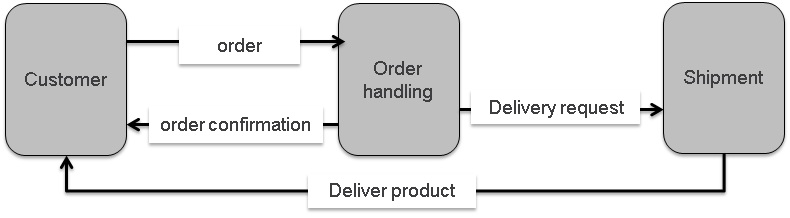
\includegraphics[width=0.7\linewidth]{Figures/Ontology/SubjectExecution/OrderComStructure}
	\caption[The Communication Structure in the Order Process]{The Communication Structure in the Order Process}
	\label{fig:ordercomstructure}
\end{figure}

Each subject has a so-called input pool which is its mailbox for receiving messages. This input pool can be structured according to the business requirements at hand. The modeler can define how many messages of which type and/or from which sender can be deposited and what the reaction is if these restrictions are violated. This means the synchronization through message exchange can be specified for each subject individually.

Messages have an intuitive meaning expressed by their name. A formal semantics is given by their use and the data which are transported with a message. Figure \ref{fig:ordercustomerorderhandling} depicts the behavior of the subjects "customer" and "order handling".

%\strictpagecheck
\begin{figure}[htbp]
	\centering
	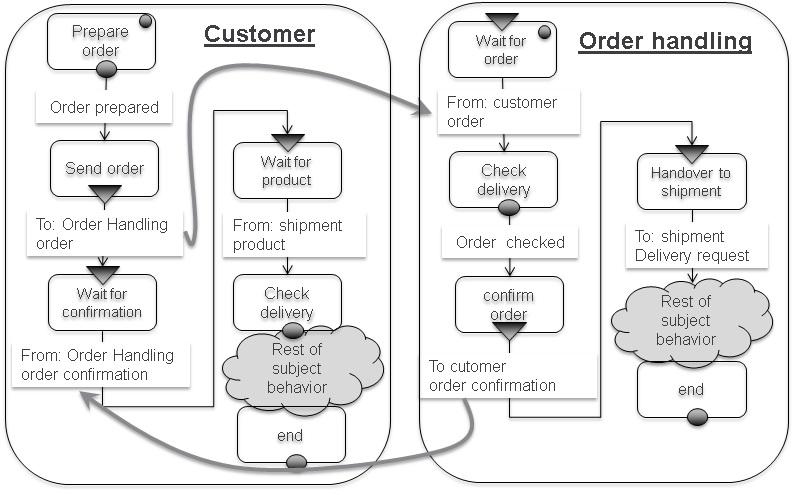
\includegraphics[width=0.9\linewidth]{Figures/Ontology/SubjectExecution/OrderCustomerOrderHandling}
	\caption[The Behavior of Subjects]{The Behavior of Subjects}
	\label{fig:ordercustomerorderhandling}
\end{figure}

In the first state of its behavior, the subject "customer" executes the internal function "Prepare order". When this function is finished the transition "order prepared" follows. In the succeeding state "send order" the message "order" is sent to the subject "order handling". After this message is sent (deposited in the input pool of subject "order handling"), the subject "Customer" goes into the state "wait for confirmation". If this message is not in the input pool the subject stops its execution until the corresponding message arrives in the input pool. On arrival, the subject removes the message from the input pool and follows the transition into state "Wait for product" and so on.

The subject "Order Handling" waits for the message "order" from the subject "customer". If this message is in the input pool it is removed and the succeeding function "check order" is executed and so on.

The behavior of each subject describes in which order it sends messages, expects (receives) and performs internal functions. Messages transport data from the sending to the receiving subject and internal functions operate on internal data of a subject. These data aspects of a subject are described in section \ref{SUbjects-Objects}. In a dynamic and fast-changing world, processes need to be able to capture known but unpredictable events. In our example let us assume that a customer can change an order. This means the subject "customer" may send the message "Change order" at any time. Figure \ref{fig:ordercomstructure} shows the corresponding communication structure, which now contains the message "change order".

%\strictpagecheck
\begin{figure}[htbp]
	\centering
	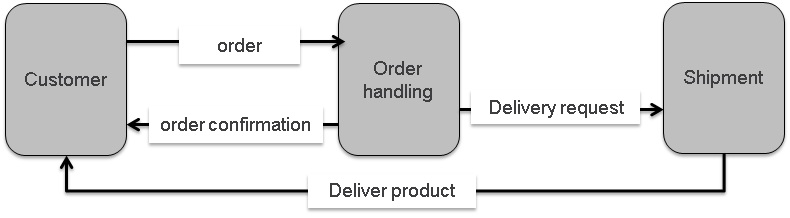
\includegraphics[width=0.7\linewidth]{Figures/Ontology/SubjectExecution/OrderComStructure}
	\caption[The Communication Structure with Change Message]{The Communication Structure with Change Message}
	\label{fig:ordercomstructure}
\end{figure}

Due to this unpredictable event, the behavior of the involved subjects needs also to be adapted. Figure \ref{fig:ordercustomerchange} illustrates the respective behavior of the customer. 

%\strictpagecheck
\begin{figure}[htbp]
	\centering
	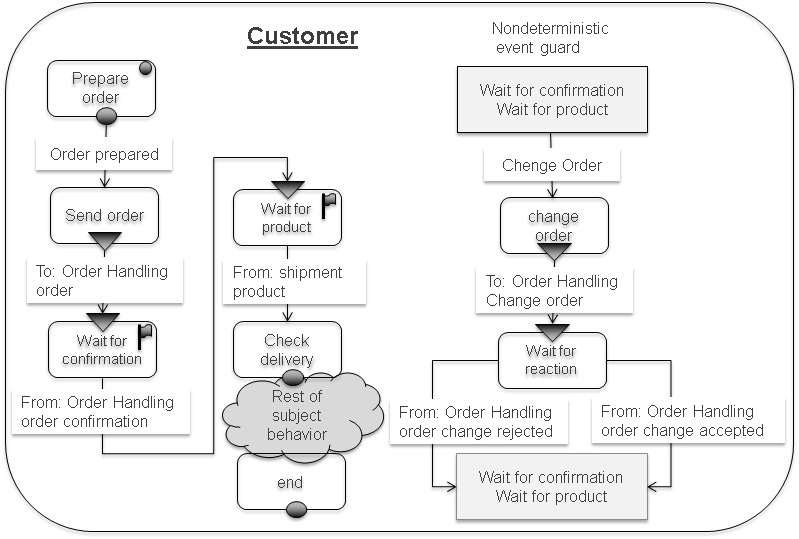
\includegraphics[width=0.9\linewidth]{Figures/Ontology/SubjectExecution/OrderCustomerChange}
	\caption[Customer is allowed to Change Orders]{Customer is allowed to Change Orders}
	\label{fig:ordercustomerchange}
\end{figure}

The subject "customer" may have the idea to change its order in the state "wait for confirmation" or in the state "wait for product". The flags in these states indicate that there is a so-called behavior extension described by a so-called nondeterministic event guard [12, 22]. The non-deterministic event created in the subject is the idea "change order". If this idea comes up, the current states, either "wait for confirmation" or "wait for product", are left, and the subject "customer" jumps into state "change order" in the guard behavior. In this state, the message "change order" is sent and the subject waits in the state "wait for reaction". In this state, the answer can either be "order change accepted" or "order change rejected". Independently of the received message the subject "customer" moves to the state "wait for product". The message "order change accepted" is considered as confirmation, if a confirmation has not arrived yet (state "wait for confirmation"). If the change is rejected the customer has to wait for the product(s) he/she has ordered originally. Similar to the behavior of the subject "customer" the behavior of the subject "order handling" has to be adapted.

\subsection{Subjects and Objects}
\label{SUbjects-Objects}

Up to now, we did not mention data or the objects with their predicates, to get complete sentences comprising subject, predicate, and object. Figure \ref{fig:subjectobject} displays how subjects and objects are connected. The internal function "prepare order" uses internal data to prepare the data for the order message. This order data is sent as the payload of the message "order".

%\strictpagecheck
\begin{figure}[htbp]
	\centering
	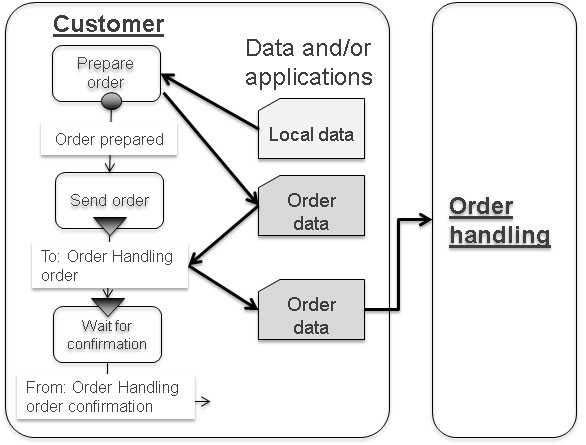
\includegraphics[width=0.9\linewidth]{Figures/Ontology/SubjectExecution/SUbjectObject}
	\label{fig:subjectobject}
	\caption[Subjects and Objects]{Subjects and Objects}
\end{figure}

The internal functions in a subject can be realized as methods of an object or functions implemented in a service if a service-oriented architecture is available. These objects have an additional method for each message. If a message is sent, the method allows receiving data values sent with the message, and if a message is received the corresponding method is used to store the received data in the object [22]. This means either subject are the entities which use synchronous services as an implementation of functions or asynchronous services are implemented through subjects or even through complex processes consisting of several subjects. Consequently, the concept Service Oriented Architecture (SOA) is complementary to S-BPM: Subjects are the entities which use the services offered by SOAs (cf. [25]).

\section{Introduction to Ontologies and OWL }
\label{IntroOntology}

This short introduction to ontology, the Resource Description Framework and Web Ontology Language (OWL), should help to get an understanding of the PASS ontology outlined in section \ref{PASSStruct} and \ref{PASSExec}.

Ontologies are a formal way to describe taxonomies and classification networks, essentially defining the structure of knowledge for various domains: the nouns representing classes of objects and the verbs representing relations between the objects of classes.

In computer science and information science, an ontology encompasses a representation, formal naming, and definition of the classes, properties, and relations between the data, and entities that substantiate considered domains.

The Resource Description Framework (RDF) provides a graph-based data model or framework for structuring data as statements about resources. A "resource" may be any "thing" that exists in the world: a person, place, event, book, museum object, but also an abstract concept like data objects. Figure \ref{fig:classes-properties}  shows an RDF graph.

%\strictpagecheck
\begin{figure}[h]
	\centering
	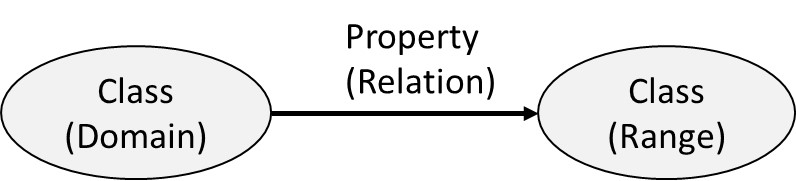
\includegraphics[width=0.6\linewidth]{Figures/Ontology/Introduction/Classes-Properties}
	\caption[RDF graphic]{RDF graphic}
	\label{fig:classes-properties}
\end{figure}

RDF is based on the idea of making statements about resources (in particular web resources) in expressions of the form subject–predicate–object, known as triples. The subject denotes the resource, and the predicate denotes traits or aspects of the resource and expresses a relationship between the subject and the object. In the context of ontology, the term subject expresses what the sentence is about (topic) (see \ref{SubjectOrient}).

For describing ontologies several languages have been developed. One widely used language is OWL (worldwide web ontology language) which is based on the Resource Description Framework (RDF).

OWL has classes, properties, and instances. Classes represent terms also called concepts. Classes have properties and instances are individuals of one or more classes.

A class is a type of thing. A type of "resource" in the RDF sense can be
person, place, object, concept, event, etc.. Classes and subclasses form a hierarchical taxonomy and members of a subclass inherit the characteristics of their parent class (superclass). Everything true for the parent class is also true for the subclass.

A member of a subclass "is a", or "is a kind of" its parent class. Ontologies define a set of properties used in a specific knowledge domain. In an ontology context, properties relate members of one class to members of another class or a literal.

Domains and ranges define restrictions on properties. A domain restricts what kinds of resources or members of a class can be the subject of a given property in an RDF triple. A range restricts what kinds of resources/members of a class or data types (literals) can be the object of a given property in an RDF triple.

Entities belonging to a certain class are instances of this class or individuals. A simple ontology with various classes, properties and individual is shown below:

Ontology statement examples:

\begin{itemize}
	\item \textbf {Class definition statements:}
	\begin{itemize}
		\item Parent \texttt{isA} Class
		\item Mother \texttt{isA} Class
		\item Mother \texttt{subClassOf} Parent
		\item Child \texttt{isA} Class
	\end{itemize}
	\item \textbf {Property definition statement:}
	\begin{itemize}
		\item \texttt{isMotherOf} is a relation between the classes Mother and Child
	\end{itemize}
	\item \textbf{Individual/instance statements:}
	\begin{itemize}
		\item MariaSchmidt \texttt{isA} Mother
		\item MaxSchmidt \texttt{isA} Child
		\item MariaSchmidt \texttt{isMotherOf} MaxSchmidt
	\end{itemize}
\end{itemize}

\section{Introduction to Abstract State Machines }

An abstract state machine (ASM) is a state machine operating on states that are arbitrary data structures (structure in the sense of mathematical logic, that is a nonempty set together with several functions (operations) and relations over the set).

The language of the so-called Abstract State Machine uses only elementary If-Then-Else-rules which are typical also for rule systems formulated in natural language, i.e., rules of the (symbolic) form 

\medskip
\textbf{if} \textit{Condition} \textbf{then} \textit{ACTION}
\medskip

with arbitrary \textit{Condition} and \textit{ACTION}. The latter is usually a finite set of assignments of the form \textit{f (t1, ..., tn) := t}. The meaning of such a rule is to perform in any given state the indicated action if the indicated condition holds in this state.

The unrestricted generality of the used notion of Condition and \textit{ACTION} is guaranteed by using as ASM-states the so-called Tarski structures, i.e., arbitrary sets of arbitrary elements with arbitrary functions and relations defined on them. These structures are updatable by rules of the form above. In the case of business processes, the elements are placeholders for values of arbitrary type and the operations are typically the creation, duplication, deletion, or manipulation (value change) of objects. The so-called views are conceptually nothing else than projections (read: substructures) of such Tarski structures.

An (asynchronous, also called distributed) ASM consists of a set of agents each of which is equipped with a set of rules of the above form, called its program. Every agent can execute in an arbitrary state in one step all its executable rules, i.e., whose condition is true in the indicated state. For this reason, such an ASM, if it has only one agent, is also called sequential ASM. In general, each agent has its own "time" to execute a step, in particular, if its step is independent of the steps of other agents;  in special cases, multiple agents can also execute their steps simultaneously (in a synchronous manner).

Without further explanations, we adopt usual notations, abbreviations, etc., for example:

% for the typesetting of ASM code some work is required!!

%\lstdefinelanguage{ASM}{C}
%\lstset{language=ASM}

\begin{lstlisting}
if Cond then M1 else M2
\end{lstlisting}

instead of the equivalent ASM with two rules:

\begin{lstlisting}
if Cond then M1
if not Cond then M2
\end{lstlisting}

Another notation used below is

\begin{lstlisting}
let x=t in M
\end{lstlisting}

for $M(x/a)$, where $a$ denotes the value of $t$ in the given state and $M(x/a)$ is obtained from $M$ by substitution of each (free) occurrence of $x$ in $M$ by $a$.

For details of a mathematical definition of the semantics of ASMs which justifies their intuitive (rule-based or pseudo-code) understanding, we refer the reader to the AsmBook Börger, E., Stärk R. Abstract State Machines. A Method for High-Level System Design and Analysis. Springer, 2003.






\chapter{Structure of a PASS Description}
\label{PASSStruct}
	In this chapter we describe the structure of a PASS specification. The structure of a PASS descritption consists of the subjects and the messages they exchange.

\section{Informal Description}
\subsection{Subject}
\label{sec: Subject}

Subjects represent the behavior of an active entity. A specification of a subject does not say anything about the technology used to execute the described behavior. 
Subjects communicate with each other by exchanging messages. Messages have a name and a payload. The name should express the meaning of a message informally and the payloads are the data (business objects) transported. Internally subjects execute local activities such as calculating a price, storing an address etc.
A subject sends messages to other subjects, expects messages from other subjects, and executes internal actions. All these activities are done in sequences which are defined in a subject's behavior specification.

In the following we use an example for the informal definiton of subjects.\
In the simple scenario of the business trip application, we can identify three subjects, namely the employee as applicant, the manager as the approver, and the travel office as the travel arranger.

There are the following types of subjects:
\begin{itemize}
	\item Fully specified subjects 
	\item Multisubjects 
	\item Single subject
	\item Interface subjects 
\end{itemize}

\subsubsection{Fully specified Subjects}
This is the standard subject type. A subject communicates with other subjects by exchangeing messages.
Fully specified subjects consists of following components:
\begin{itemize}
	\item Business Objects\\
	Each subjects has some business objects. A basic structure of business objects consists of an identifier, data structures, and data elements. The identifier of a business object is derived from the business environment in which it is used. Examples are business trip requests, purchase orders, packing lists, invoices, etc.
	Business objects are composed of data structures. Their components can be simple data elements of a certain type (e.g., string or number) or even data structures themselves. 
	\item Sent messages\\
	Messages which a subject sends to other subjects. Each message has a name and may transport some data objects as a payload. The values of these payload data objects are copied from internal business objects of a subject.
	\item Received messages\\
	Messages received by a subject. The values of the payload objects are copied to business objects of the receiving subject.
	\item Input Pool\\
	Messages sent to a subjects are deposited in the input pool of the receiving subject.
	\item Behavior \\
	The behavior of each subject describes in which order it sends messages, expects (receives) and performs internal functions. Messages transport data from the sending to the receiving subject, and internal functions operate on internal data of a subject. 
\end{itemize}


\subsubsection{Multsubjects and Multiprocesses}
Multisubjects are simular to Fully specified subjects. If in a process model several identical subjects are required e.g. in order to increse the through put these subjects can be modelled by a multi subject. If several communicating subjects in a process modell are multi subjects they can be combined to a multi process.

In a business process, there may be several identical sub-processes that perform certain similar tasks in parallel and independently. This is often the case in a procurement process, when bids from multiple providers are solicited. A process or sub-process is therefore executed simultaneously or sequentially multiple times during overall process execution. A set of type-identical, independently running processes or sub-processes are termed multi-process. The actual number of these independent sub-processes is determined at runtime.
Multi-processes simplify process execution, since a specific sequence of actions can be used by different processes. They are recommended for recurring structures and similar process flows.
An example of a multi-process can be illustrated as a variation of the current booking process. The travel agent should simultaneously solicit up to five bids before making a reservation. Once three offers have been received, one is selected and a room is booked. The process of obtaining offers from the hotels is identical for each hotel and is therefore modeled as a multi-process.


\subsubsection{Single subjects}
Single subjects can be instantiated only once. They are used if for the execution of a subject a resource is required which is only available once.


\subsubsection{Interface Subjects}
Interface subjects are used as interfaces to other process systems. If a subject of a process system sends or receives messages from a subject which belongs to an other process system. These so called interface subjects represent fully described subjects which belong to that other process system. This means to each interface subject belongs a fully described subject in an other process system. Interface subjects specifications contain the sent messages, received messages and the refernce to the fully described subject which they represent.


\subsection{Subject-to-Subject Communication}
After the identification of subjects involved in the process (as process-specific roles), their interaction relationships need to be represented. These are the messages exchanged between the subjects. Such messages might contain structured information—so-called business objects (see Section xxxxxxx).\

The result is a model structured according to subjects with explicit communication relationships, which is referred to as a Subject Interaction Diagram (SID) or, synonymously, as a Communication Structure Diagram (CSD) (see figure \ref{fig:beispiel-subject-interaction}).

\begin{figure*}[ph]
	\centering
	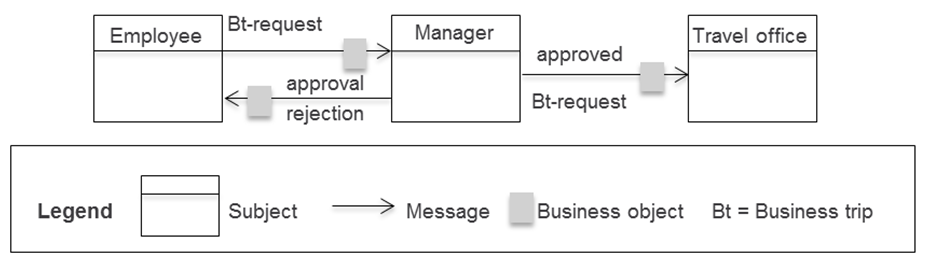
\includegraphics[width=14cm]{20181026-Ontologie-Bilder/Grafiken-Ontologie/SUbject-Interaction/Beispiel-Subject-Interaction}
	\caption[Subject interaction diagram]{Subject interaction diagram for the process ‘business trip application’}
	\label{fig:beispiel-subject-interaction}
\end{figure*}


Messages represent the interactions of the subjects during the execution of the process. We recommend naming these messages in such a way that they can be immediately understood and also reflect the meaning of each particular message for the process. In the sample ‘business trip application’, therefore, the messages are referred to as ‘business trip request’, ‘rejection’, and ‘approval’.

Messages serve as a container for the information transmitted from a sending to a receiving subject. There are two options for the message content:

\begin{itemize}
	\item 	Simple data types: Simple data types are string, integer, character, etc. In the business trip application example, the message ‘business trip request’ can contain several data elements of type string (e.g., destination, reason for traveling, etc.), and of type number (e.g., duration of trip in days).
	\item Business Objects: Business Objects in their general form are physical and logical ‘things’ that are required to process business transactions., We consider data structures composed of elementary data types, or even other data structures, as logical business objects in business processes. For instance, the business object ‘business trip request’ could consist of the data structures ‘data on applicants’, ‘travel data’, and ‘approval data’—with each of these in turn containing multiple data elements.
\end{itemize}


\subsection{Message Exchange}

In the previous subsection, we have stated that messages are transferred between subjects and have described the nature of these messages. What is still missing is a detailed description of how messages can be exchanged, how the information they carry can be transmitted, and how subjects can be synchronized. These issues are addressed in the following sub-sections.

\subsubsection{Synchronous and Asynchronous Exchange of Messages}
In the case of synchronous exchange of messages, sender and receiver wait for each other until a message can be passed on. If a subject wants to send a message and the receiver (subject) is not yet in a corresponding receive state, the sender waits until the receiver is able to accept this message. Conversely, a recipient has to wait for a desired message until it is made available by the sender.\

The disadvantage of the synchronous method is a close temporal coupling between sender and receiver. This raises problems in the implementation of business processes in the form of workflows, especially across organizational borders. As a rule, these also represent system boundaries across which a tight coupling between sender and receiver is usually very costly. For long-running processes, sender and receiver may wait for days, or even weeks, for each other.\

Using asynchronous messaging, a sender is able to send anytime. The subject puts a message into a message buffer from which it is picked up by the receiver. However, the recipient sees, for example, only the oldest message in the buffer and can only accept this particular one. If it is not the desired message, the receiver is blocked, even though the message may already be in the buffer, but in a buffer space that is not visible to the receiver. To avoid this, the recipient has the alternative to take all of the messages from the buffer and manage them by himself. In this way, the receiver can identify the appropriate message and process it as soon as he needs it. In asynchronous messaging, sender and receiver are only loosely coupled. Practical problems can arise due to the in reality limited physical size of the receive buffer, which does not allow an unlimited number of messages to be recorded. Once the physical boundary of the buffer has been reached due to high occupancy, this may lead to unpredictable behavior of workflows derived from a business process specification. To avoid this, the input-pool concept has been introduced in PASS.


\subsubsection{Exchange of Messages via the Input Pool}
\label{sec: inputpool}
To solve the problems outlined in asynchronous message exchange, the input pool concept has been developed. Communication via the input pool is considerably more complex than previously shown; however, it allows transmitting an unlimited number of messages simultaneously. Due to its high practical importance, it is considered as a basic construct of PASS.
Consider the input pool as a mail box of work performers, the operation of which is specified in detail.
Each subject has its own input pool. It serves as a message buffer to temporarily store messages received by the subject, independent of the sending communication partner. The input pools are therefore inboxes for flexible configuration of the message exchange between the subjects. In contrast to the buffer in which only the front message can be seen and accepted, the pool solution enables picking up (= removing from the buffer) any message. For a subject, all messages in its input pool are visible.

The input pool has the following configuration parameters (see figure \ref{fig:input-pool}):\
\begin{itemize}
	\item Input-pool size: The input-pool size specifies how many messages can be stored in an input pool, regardless of the number and complexity of the message parameters transmitted with a message. If the input pool size is set to zero, messages can only be exchanged synchronously.
	\item Maximum number of messages from specific subjects: For an input pool, it can be determined how many messages received from a particular subject may be stored simultaneously in the input pool. Again, a value of zero means that messages can only be accepted synchronously.
	\item Maximum number of messages with specific identifiers: For an input pool, it can be determined how many messages of a specifically identified message type (e.g., invoice) may be stored simultaneously in the input pool, regardless of what subject they originate from. A specified size of zero allows only for synchronous message reception.
	\item Maximum number of messages with specific identifiers of certain subjects: For an input pool, it can be determined how many messages of a specific identifier of a particular subject may be stored simultaneously in the input pool. The meaning of the zero value is analogous to the other cases.
\end{itemize}
\newpage
\begin{figure*}[ph]
	\centering
	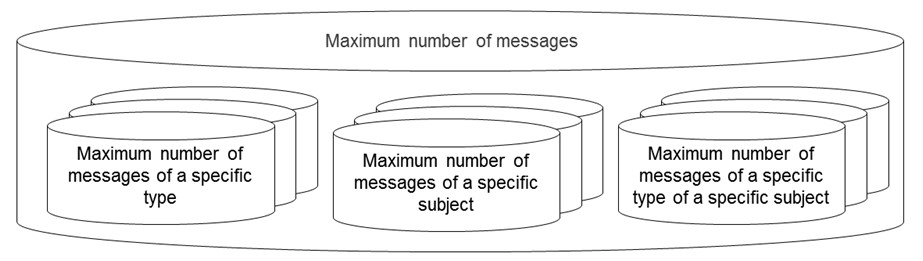
\includegraphics[width=12cm]{20181026-Ontologie-Bilder/Grafiken-Ontologie/SUbject-Interaction/input-pool-informal.jpg}
	\caption[Input Pool]{Configuration of Input Pool Parameters}
	\label{fig:input-pool}
\end{figure*}


By limiting the size of the input pool, its ability to store messages may be blocked at a certain point in time during process runtime. Hence, messaging synchronization mechanisms need to control the assignment of messages to the input pool. Essentially, there are three strategies to handle the access to input pools:
\begin{itemize}
	\item Blocking the sender until the input pool’s ability to store messages has been reinstated: Once all slots are occupied in an input pool, the sender is blocked until the receiving subject picks up a message (i.e. a message is removed from the input pool). This creates space for a new message. In case several subjects want to put a message into a fully occupied input pool, the subject that has been waiting longest for an empty slot is allowed to send. The procedure is analogous if corresponding input pool parameters do not allow storing the message in the input pool, i.e., if the corresponding number of messages of the same name or from the same subject has been put into the input pool.
	\item Delete and release of the oldest message: In case all the slots are already occupied in the input pool of the subject addressed, the oldest message is overwritten with the new message.
	\item Delete and release of the latest message: The latest message is deleted from the input pool to allow depositing of the newly incoming message. If all the positions in the input pool of the addressed subject are taken, the latest message in the input pool is overwritten with the new message. This strategy applies analogously when the maximum number of messages in the input pool has been reached, either with respect to sender or message type.
\end{itemize}

\newpage

\section{OWL Description}

The various building blocks of a PASS description and their relations are defined in a ontology. The following figure \ref{fig:20171217-passprocessmodellelement} gives an overview of the structure of PASS specifications.   

\begin{figure*}[ph]
	\centering
	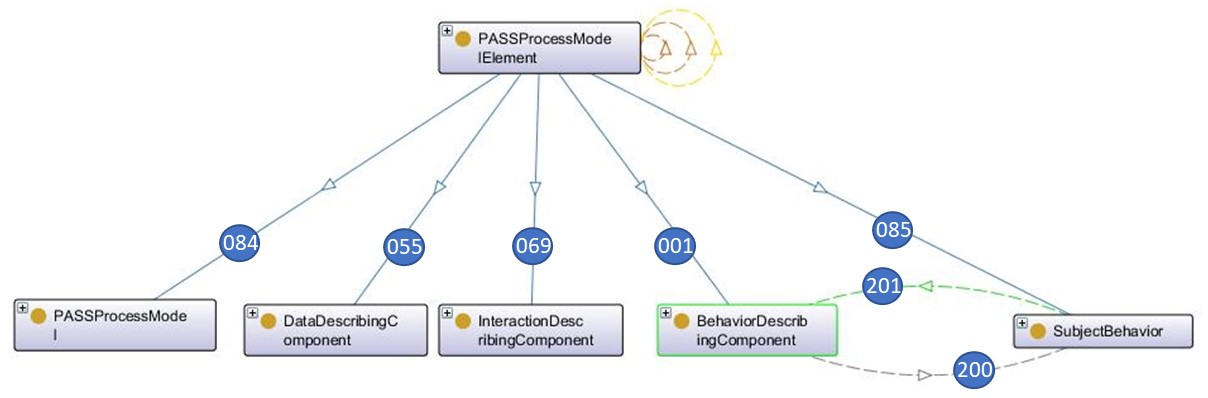
\includegraphics[width=0.9\linewidth]{20181026-Ontologie-Bilder/Grafiken-Ontologie/SUbject-Interaction/20171217-PASSProcessModellElement}
	\caption[Elements of PASS Process Models]{Elements of PASS Process Models}
	\label{fig:20171217-passprocessmodellelement}
\end{figure*}

The class PASSProcessModelElement hs 5 subclasses (subclass relations 084, 055, 069, 001 an 085 in figure \ref{fig:20171217-passprocessmodellelement}). Only the classes PASSProcessModel, DataDescriptionCOmponent, InteractionDescribingComponent are used for defining the structural aspects of a process specification in PASS. The classes BehaviorDescribingComponent and SUbject Behavior define the dynamic aspects. In which sequences messages are sent and received or internal actions are executed. These dynamic asoects are considered in detail in Chapter 3. 



\subsection{PASS Process Model}
The central entities of a PASS process model are subjects which represents the active elements of a process and the messages they exchange. Messages transport data from one subject to others (payload). The following figure \ref{fig:20181217-passprocessmodel} shows the coresponding ontology for the PASS Process models.

\begin{figure*}[ph]
	\centering
	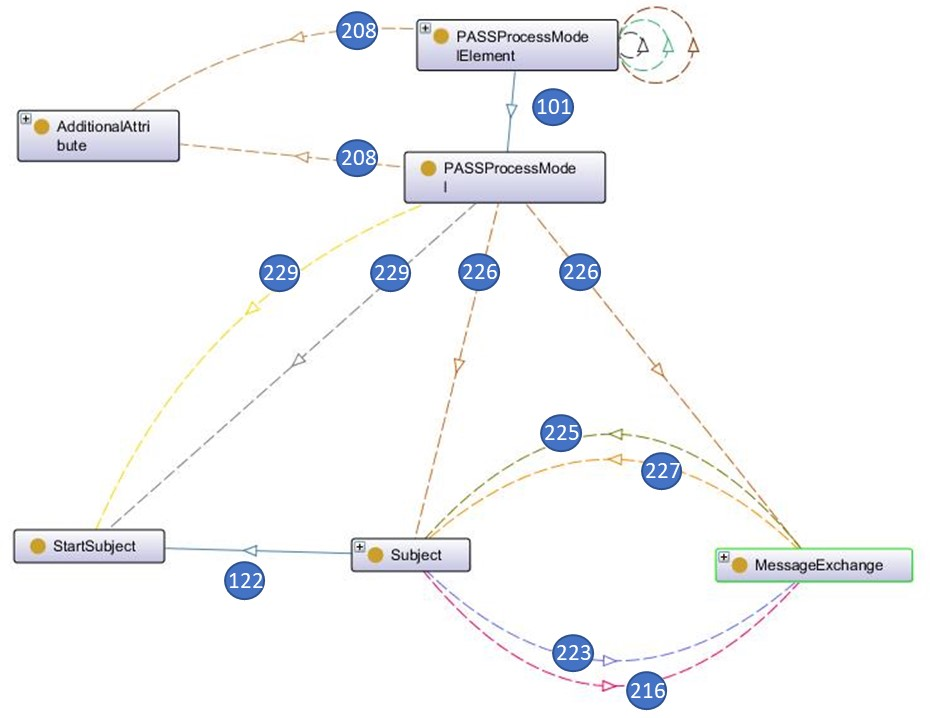
\includegraphics[width=1.0\linewidth]{20181026-Ontologie-Bilder/Grafiken-Ontologie/SUbject-Interaction/20181217-PASSProcessModel}
	\caption[PASS Process Modell]{PASS Process Modell}
	\label{fig:20181217-passprocessmodel}
\end{figure*}

PASSProcessModelElements and PASSProcessModells have a name. This is described with the property hasAdditionalAttribute (property 208 in \ref{fig:20171217-passprocessmodellelement}). The class subject and the class MessageExchange have the relation hasRelationtoModelComponent to the class PASSProcessModel (property 226 in \ref{fig:20171217-passprocessmodellelement}). The properties hasReceiver and hasSender express that a message has a sending and receiving subject (properties 225 and 227 in \ref{fig:20171217-passprocessmodellelement}) whereas the properties hasOutgoingMessageExchange and hasIncomingMessageExchange define which messages are sent or received by a subject. Property hasStartSubject (property 229 in \ref{fig:20171217-passprocessmodellelement}) defines a start subject for a PASSProcessModell. A start subject is a subclass of the class subject (subclass relation 122 in \ref{fig:20171217-passprocessmodellelement}).


\subsection{Data Describing Component}
Each subject encapsulate data (business objects). The values of these data elements can be transfered to other subjects. The following figure \ref{fig:20181218-data} shows the ontology of this part of the PASS-ontology.

\begin{figure}[ph]
	\centering
	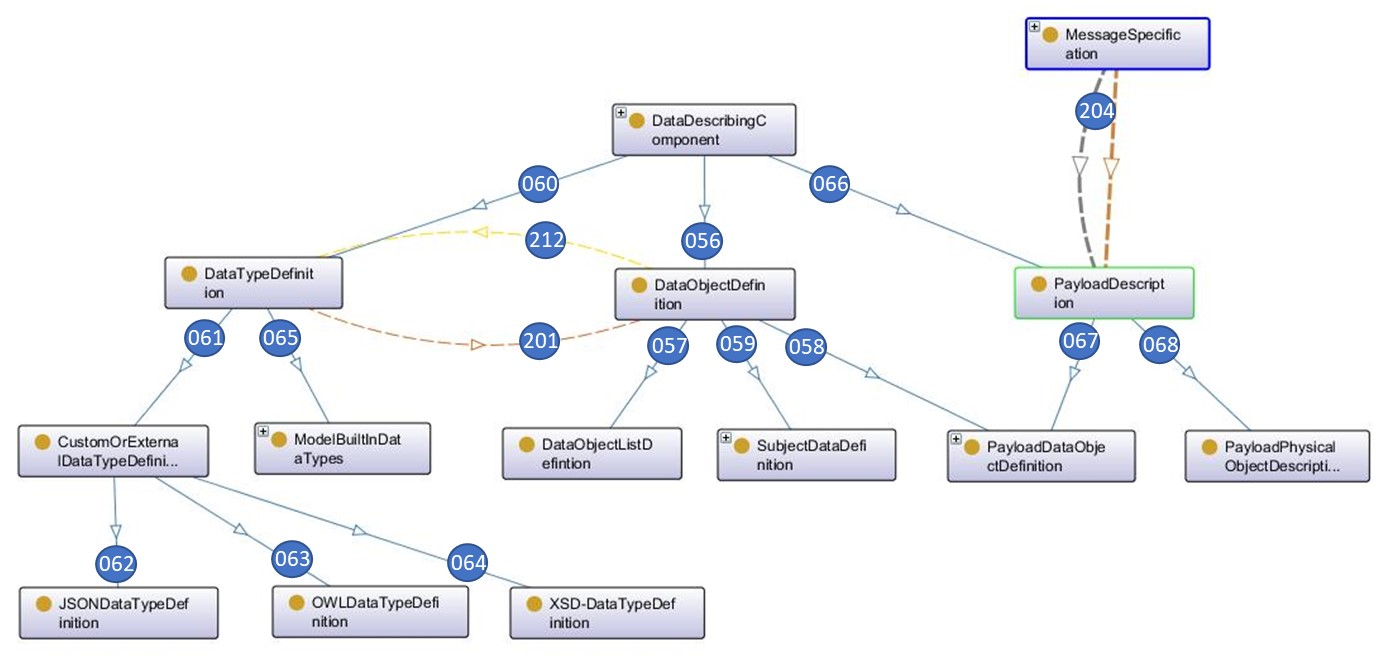
\includegraphics[width=0.9\linewidth]{20181026-Ontologie-Bilder/Grafiken-Ontologie/SUbject-Interaction/20181218-Data}
	\caption[Data Description Component]{Data Description Component}
	\label{fig:20181218-data}
\end{figure}

From class DtadescribingCombonent three subclasses are derived (in figure \ref{fig:20181218-data} are these the relations 060, 056 and 066). Subclass PayLoadDescription are the data tranported by messages.he relation of PayloadDescriptions to messages is defined by property ContainsPayloadDescription (in figure \ref{fig:20181218-data} number 204). \\
There are two types of payloads. The class PayloadPhysicalObjectDescription is used if a message will be later implemented by a physical transport like a parcel. The class PayLoadDataObjectDefinition is used to transport normal data (Subclass relations 068 and 67 in figure \ref{fig:20181218-data}). These payload objects are also a subclass of class DataObjectDefinition (Subclass relation 058 in figure \ref{fig:20181218-data}). \\
Data objects have a certain type. Therefore class DataObjectDefinition has the relation hasDatatype to class DataTypeDefinition (property 212 in figure\ref{fig:20181218-data}). Class DataTypeDefinition has two subclasses (subclass relations 061 and 065 in figure \ref{fig:20181218-data}). The subclass ModelBuiltInDataTypes are user defined data types whereas the class CustomOfExternalDataTypeDefinition is the superclass of JSON, OWL or XML based data type definitions(subclass relations 062, 63 and 064 in figure \ref{fig:20181218-data}).

\newpage

\subsection{Interaction Describing Component}

The following figure \ref{fig:ontogrsubjectinteraction} shows the subset of the classes and properties required for describing the interaction of subjects. 

\begin{figure*}[ph]
	\centering
	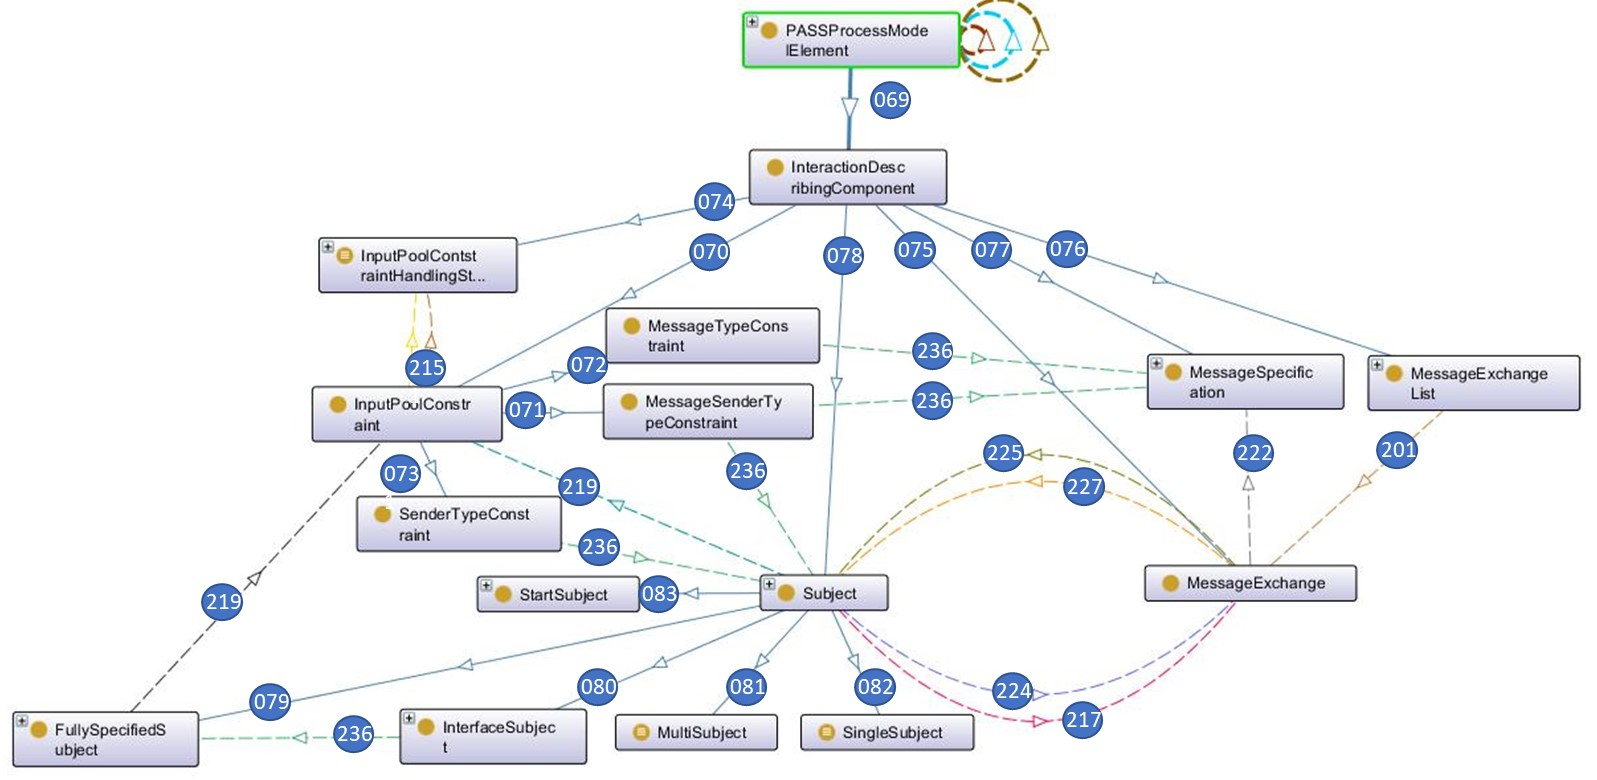
\includegraphics[width=1.0\linewidth]{20181026-Ontologie-Bilder/Grafiken-Ontologie/SUbject-Interaction/OntoGrSubjectInteraction}
	\caption[Subject Interaction Diagram]{Subject Interaction Diagram}
	\label{fig:ontogrsubjectinteraction}
\end{figure*}


The central classes are Subject and MessageExchange. Between these classes are defined the properties hasIncomingTransition (in figure \ref{fig:ontogrsubjectinteraction} number 217) and hasOutgoingTransition (in figure \ref{fig:ontogrsubjectinteraction} number 224). This properties defines that subjects have incoming and outgoing messages. Each message has a sender and a receiver (in figure \ref{fig:ontogrsubjectinteraction} number 227 and number 225). Messages have a type. This is expressed by the property hasMessageType (in figure \ref{fig:ontogrsubjectinteraction} number 222). Instead of the property 222 a message exchange may have the property 201 if a list of messages is used instead of a single message.\\
Each subject has an input pool. Input pools have three types of constraints (see section \ref{sec: inputpool}). This is expressed by the property references  (in figure \ref{fig:ontogrsubjectinteraction} number 236) and InputPoolConstraints (in figure \ref{fig:ontogrsubjectinteraction} number 219). Constraints which are related to certain messages have references to the class MessageSpecification.\\
There are four subclasses of the class subject (in figure \ref{fig:ontogrsubjectinteraction} number 079, 080, 081 and 082). The specialties of these subclasses are described in section \ref{sec: Subject}. A class StartSubject (in figure \ref{fig:ontogrsubjectinteraction} number 83) which is a subclass of class subject denotes the subject in which a process instance is started.\\
All other relarions are subclass relations. The class PASSProcessModelElement is the central PASS class. From this class all the other classes are derived (see next sections). From class InteractionDescribingCOmponent all the classes required for describing the structure of a process system are derived.

\section{ASM Description}
In this chapter only the structure of a PASS model is considered. Execution has not been considered. Because ASM only considers execution aspects in this chapter an ASM specification of the structural aspects does not make sense. The execution semantic is part of chapter 4.
\chapter{Execution of a PASS Model}
\label{PASSExec}

\section{Informal Description of Subject Behavior and its Execution}

The execution of the subject means sending and receiving messages and executing internal activities in the defined order. In the following sections, it is described what sending and receiving messages and executing internal functions means.

\subsection{Sending Messages}

Before sending a message, the values of the parameters to be transmitted need to be determined. In case the message parameters are simple data types, the required values are taken from local variables or business objects of the sending subject, respectively. In the case of business objects, a current instance of a business object is transferred as a message parameter.

The sending subject attempts to send the message to the target subject and store it in its input pool. Depending on the described configuration and status of the input pool, the message is either immediately stored or the sending subject is blocked until delivery of the message is possible.

In the sample business trip application, employees send completed requests using the message 'send business trip request' to the manager's input pool. From a send state, several messages can be sent as an alternative. The following example shows a send state in which the message M1 is sent to the subject S1, or the message M2 is sent to S2, therefore referred to as alternative sending (see Figure \ref{fig:sendstate}). It does not matter which message is attempted to be sent first. If the send mechanism is successful, the corresponding state transition is executed. In case the message cannot be stored in the input pool of the target subject, sending is interrupted automatically, and another designated message is attempted to be sent. A sending subject will thus only be blocked if it cannot send any of the provided messages.

\begin{figure}[htbp]
	\centering
	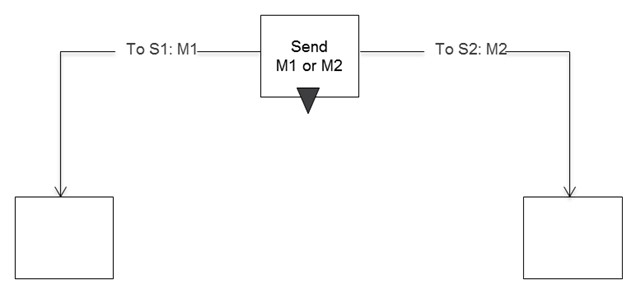
\includegraphics[width=0.7\linewidth]{20181026-Ontologie-Bilder/Grafiken-Ontologie/SUbjectExecution/sendState}
	\caption[Example of alternative sending]{Example of alternative sending}
	\label{fig:sendstate}
\end{figure}

By specifying priorities, the order of sending can be influenced. For example, it can be determined that the message M1 to S1 has a higher priority than the message M2 to S2. Using this specification, the sending subject starts with sending message M1 to S1 and then tries only in case of failure to send message M2 to S2. In case of message M2 can also not be sent to the subject S2, the attempts to send start from the beginning.

The blocking of subjects when attempting to send can be monitored over time with the so-called timeout. The example in Figure \ref{fig:sendstatetimer} shows with 'Timeout: 24 h' an additional state transition which occurs when within 24 hours one of the two messages cannot be sent. If a value of zero is specified for the timeout, the process immediately follows the timeout path when the alternative message delivery fails.

\begin{figure*}[htbp]
	\centering
	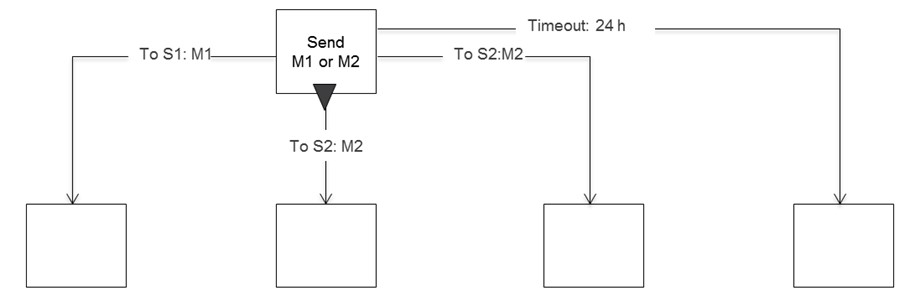
\includegraphics[width=0.7\linewidth]{20181026-Ontologie-Bilder/Grafiken-Ontologie/SUbjectExecution/SendSTateTimer}
	\caption[Send using time monitoring]{Send using time monitoring}
	\label{fig:sendstatetimer}
\end{figure*}

\subsection{Receiving Messages}

Analogously to sending, the receiving procedure is divided into two phases, which run inversely to send.

The first step is to verify whether the expected message is ready for being picked up. In the case of synchronous messaging, it is checked whether the sending subject offers the message. In the asynchronous version, it is checked whether the message has already been stored in the input pool. If the expected message is accessible in either form, it is accepted, and in a second step, the corresponding state transition is performed. This leads to a takeover of the message parameters of the accepted message to local variables or business objects of the receiving subject. In case the expected message is not ready, the receiving subject is blocked until the message arrives and can be accepted.

In a certain state, a subject can expect alternatively multiple messages. In this case, it is checked whether any of these messages are available and can be accepted. The test sequence is arbitrary unless message priorities are defined. In this case, an available message with the highest priority is accepted. However, all other messages remain available (e.g., in the input pool) and can be accepted in other receive states.

Figure \ref{fig:receivestate} shows a receive state of the subject 'employee' which is waiting for the answer regarding a business trip request. The answer may be an approval or a rejection.

\begin{figure*}[htbp]
	\centering
	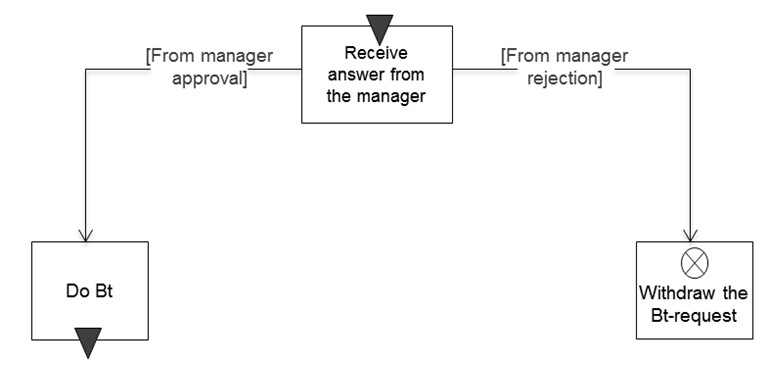
\includegraphics[width=0.7\linewidth]{20181026-Ontologie-Bilder/Grafiken-Ontologie/SUbjectExecution/ReceiveState}
	\caption[Example of alternative receiving]{Example of alternative receiving}
	\label{fig:receivestate}
\end{figure*}

Just as with sending messages, also receiving messages can be monitored over time. If none of the expected messages are available and the receiving subject is therefore blocked, a time limit can be specified for blocking. After the specified time has elapsed, the subject will execute the transition as it is defined for the timeout period. The duration of the time limit may also be dynamic, in the sense that at the end of a process instance the process stakeholders assigned to the subject decide that the appropriate transition should be performed. We then speak of a manual timeout.

\begin{figure*}[htbp]
	\centering
	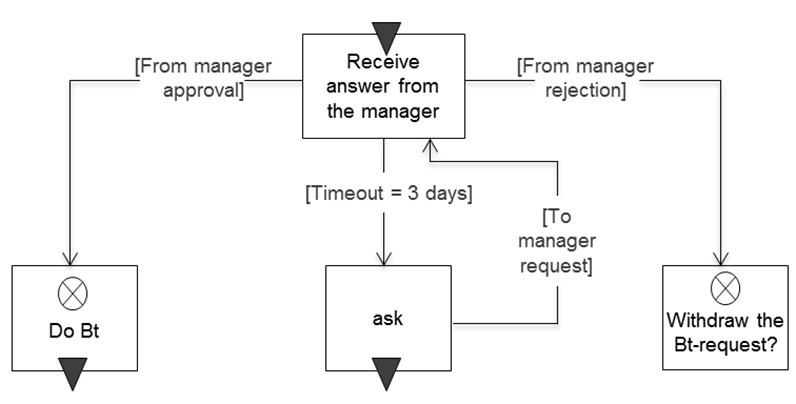
\includegraphics[width=0.7\linewidth]{20181026-Ontologie-Bilder/Grafiken-Ontologie/SUbjectExecution/ReceiveStateTimer}
	\caption[Time monitoring for message reception]{Time monitoring for message reception}
	\label{fig:receivestatetimer}
\end{figure*}

Figure \ref{fig:receivestatetimer} shows that, after waiting three days for the manager's answer, the employee sends a corresponding request.

Instead of waiting for a message for a certain predetermined period of time, the waiting can be interrupted by a subject at all times. In this case, a reason for abortion can be appended to the keyword 'breakup'. In the example shown in Figure \ref{fig:receivestatebreak}, the receiving state is left due to the impatience of the subject.

\begin{figure*}[htbp]
	\centering
	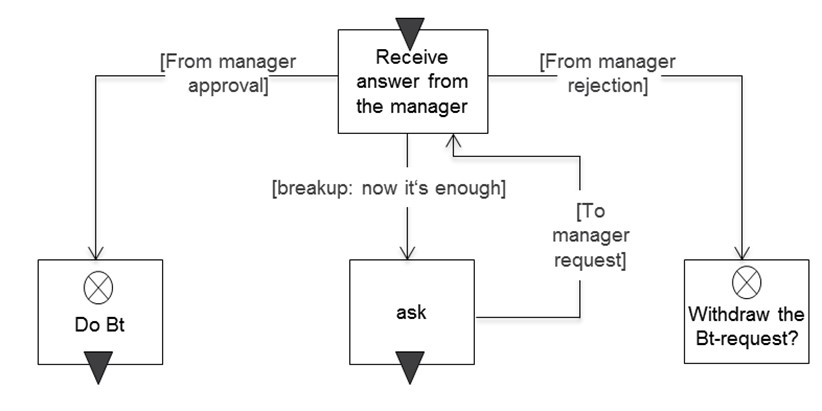
\includegraphics[width=0.7\linewidth]{20181026-Ontologie-Bilder/Grafiken-Ontologie/SUbjectExecution/ReceiveStateBreak}
	\caption[Message reception with manual interrupt]{Message reception with manual interrupt}
	\label{fig:receivestatebreak}
\end{figure*}

\subsection{Standard Subject Behavior}

The possible sequences of a subject's actions in a process are termed subject behavior. States and state transitions describe what actions a subject performs and how they are interdependent. In addition to the communication for sending and receiving, a subject also performs so-called internal actions or functions.

States of a subject are therefore distinct: There are actions on the one hand, and communication states to interact with other subjects (receive and send) on the other. This results in three different types of states of a subject. Figure \ref{fig:behavior-symbole} shows the different types of states with the corresponding symbols.

\begin{figure*}[htbp]
	\centering
	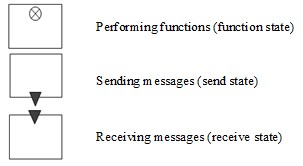
\includegraphics[width=0.5\linewidth]{20181026-Ontologie-Bilder/Grafiken-Ontologie/SUbjectExecution/Behavior-Symbole}
	\caption[State types and coresponding symbols]{State types and coresponding symbols}
	\label{fig:behavior-symbole}
\end{figure*}

In S-BPM, work performers are equipped with elementary tasks to model their work procedures: sending and receiving messages and immediate accomplishment of a task (function state).

In case an action associated with a state (send, receive, do) is possible, it will be executed, and a state transition to the next state occurs. The transition is characterized through the result of the action of the state under consideration: For a send state, it is determined by the state transition to which subject what information is sent. For a receive state, it becomes evident in this way from what subject it receives which information. For a function state, the state transition describes the result of the action, e.g., that the change of a business object was successful or could not be executed.

The behavior of subjects is represented by modelers using Subject Behavior Diagrams (SBD). Figure \ref{fig:vollst-beispiel} shows the subject behavior diagram depicting the behavior of the subjects 'employee', 'manager', and 'travel office', including the associated states and state transitions. 

\begin{landscape}
	\begin{figure}[htbp]
		\centering
		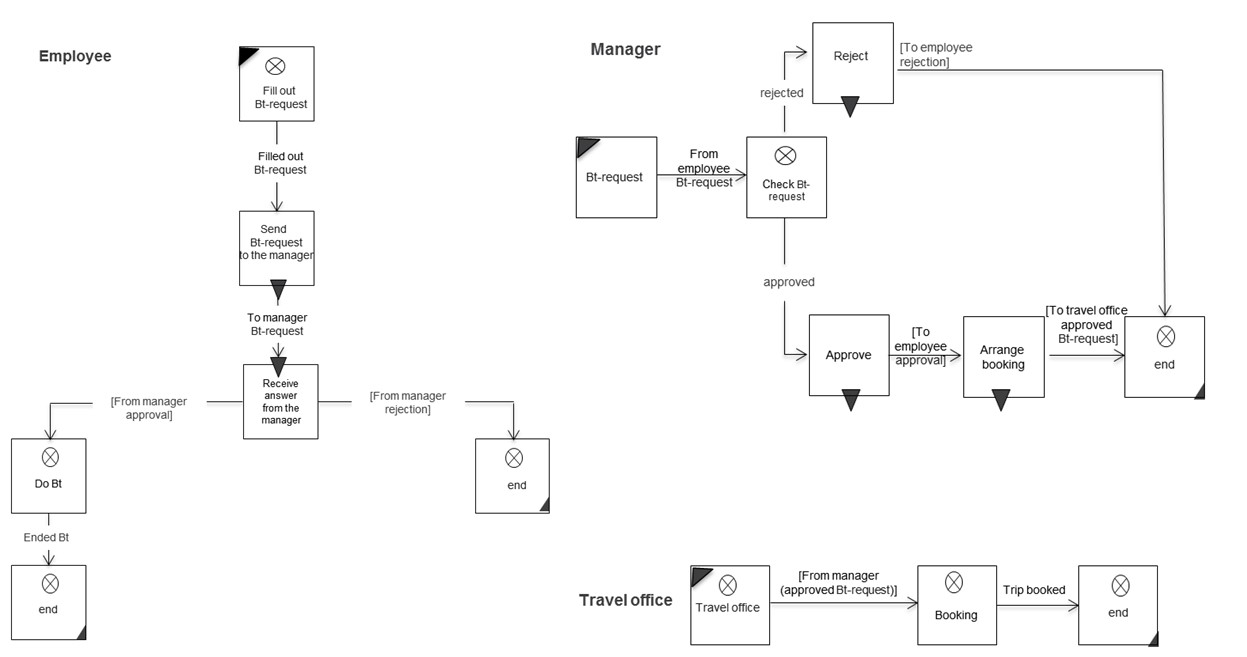
\includegraphics[width=0.9\linewidth]{20181026-Ontologie-Bilder/Grafiken-Ontologie/SUbjectExecution/Vollst-Beispiel}
		\caption[Subject behavior diagram for the subjects 'employee', 'manager', and 'travel office']{Subject behavior diagram for the subjects 'employee', 'manager', and 'travel office'}
		\label{fig:vollst-beispiel}
	\end{figure}
\end{landscape}

\subsection{Extended Behavior}

To reduce description efforts some additional specification constructs have been added to PASS. These constructs are informally explained in the following sections. 

\subsubsection{Macros}

Quite often, a certain behavior pattern occurs repeatedly within a subject. This happens in particular when in various parts of the process identical actions need to be performed. If only the basic constructs are available to this respect, the same subject behavior needs to be described many times.

Instead, this behavior can be defined as a so-called behavior macro. Such a macro can be embedded at different positions of a subject behavior specification as often as required. Thus, variations in behavior can be consolidated, and the overall behavior can be significantly simplified.

The brief example of the business trip application is not an appropriate scenario to illustrate here the benefit of the use of macros. Instead, we use an example of order processing. Figure \ref{fig:macrobehavior} contains a macro for the behavior to process customer orders. After placing the 'order', the customer receives an order confirmation; once the 'delivery' occurs, the delivery status is updated.

As with the subject, the start and end states of a macro also need to be identified. For the start states, this is done similarly to the subjects by putting black triangles in the top left corner of the respective state box. In our example, 'order' and 'delivery' are the two correspondingly labeled states. In general, this means that a behavior can initiate a jump to different starting points within a macro.

The end of a macro is depicted by gray bars, which represent the successor states of the parent behavior. These are not known during the macro definition.

\begin{figure*}[htbp]
	\centering
	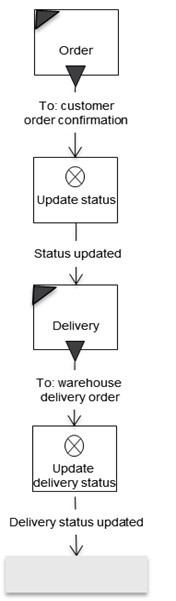
\includegraphics[width=0.2\linewidth]{20181026-Ontologie-Bilder/Grafiken-Ontologie/SUbjectExecution/MacroBehavior}
	\caption[Behavior macro class 'request for approval']{Behavior macro class 'request for approval'}
	\label{fig:macrobehavior}
\end{figure*}

Figure \ref{fig:macrousage} shows a subject behavior in which the modeler uses the macro 'order processing' to model both a regular order (with purchase order), as well as a call order.

The icon for a macro is a small table, which can contain multiple columns in the first line for different start states of the macro. The valid start state for a specific case is indicated by the incoming edge of the state transition from the calling behavior. The middle row contains the macro name, while the third row again may contain several columns with possible output transitions, which end in states of the surrounding behavior.

The left branch of the behavioral description refers to regular customer orders. The embedded macro is labeled correspondingly and started with the status 'order', namely through linking the edge of the transition 'order accepted' with this start state. Accordingly, the macro is closed via the transition 'delivery status updated'.

The right embedding deals with call orders according to organizational frameworks and frame contracts. The macro starts therefore in the state 'delivery'. In this case, it also ends with the transition 'delivery status updated'.

\begin{figure}[htbp]
	\centering
	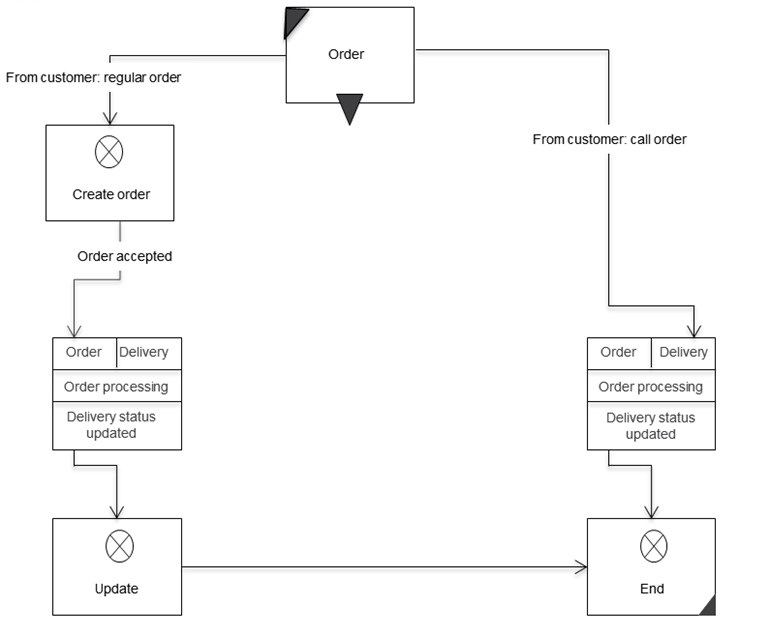
\includegraphics[width=0.6\linewidth]{20181026-Ontologie-Bilder/Grafiken-Ontologie/SUbjectExecution/MacroUsage}
	\caption[Subject behavior for order processing with macro integration]{Subject behavior for order processing with macro integration}
	\label{fig:macrousage}
\end{figure}

Similar subject behavior can be combined into macros. When being specified, the environment is initially hidden, since it is not known at the time of modeling.

\subsubsection{Guards: Exception Handling and Extensions} 

\textbf{Exception Handling}---
Handling of an exception (also termed message guard, message control, message monitoring, message observer) is a behavioral description of a subject that becomes relevant when a specific, exceptional situation occurs while executing a subject behavior specification. It is activated when a corresponding message is received, and the subject is in a state in which it can respond to the exception handling. In such a case, the transition to exception handling has the highest priority and will be enforced.

Exception handling is characterized by the fact that it can occur in a process in many behavior states of subjects. The receipt of certain messages, e.g., to abort the process, always results in the same processing pattern. This pattern would have to be modeled for each state in which it is relevant. Exception handling causes high modeling effort and leads to complex process models since from each affected state a corresponding transition has to be specified. To prevent this situation, we introduce a concept similar to exception handling in programming languages or interrupt handling in operating systems.

To illustrate the compact description of exception handling, we use again the service management process with the subject 'service desk' introduced in section 5.6.5. This subject identifies a need for a business trip in the context of processing a customer order—an employee needs to visit the customer to provide a service locally. The subject 'service desk' passes on a service order to an employee. Hence, the employee issues a business trip request. In principle, the service order may be canceled at any stage during processing up to its completion. Consequently, this also applies to the business trip application and its subsequent activities.

Below, it is first shown how the behavior modeling looks without the concept of exception handling. The cancellation message must be passed on to all affected subjects to bring the process to a defined end. Figure \ref{fig:sid-exception} shows the communication structure diagram with the added cancellation messages to the involved subjects.

\begin{figure}[ph!]
	\centering
	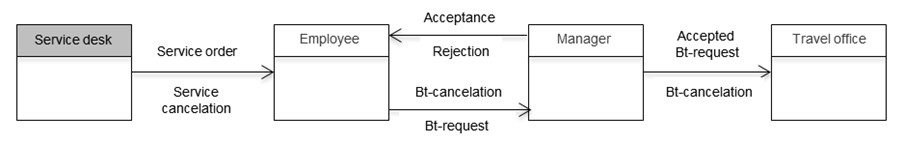
\includegraphics[width=0.7\linewidth]{20181026-Ontologie-Bilder/Grafiken-Ontologie/SUbjectExecution/SID-Exception}
	\caption[Communication structure diagram (CSD) of the business trip application]{Communication structure diagram (CSD) of the business trip application}
	\label{fig:sid-exception}
\end{figure}

A cancellation message can be received by the employee either while filling out the application or while waiting for the approval or rejection message from the manager. Concerning the behavior of the subject 'employee', the state 'response received from manager' must also be enriched with the possible input message containing the cancellation and the associated consequences (see Figure \ref{fig:exceptionhandling}). The verification of whether filing the request is followed by a cancellation is modeled through a receive state with a timeout. In case the timeout is zero, there is no cancellation message in the input pool and the business trip request is sent to the manager. Otherwise, the manager is informed of the cancellation and the process terminates for the subject 'employee'.


\begin{figure}[htbp]
	\centering
	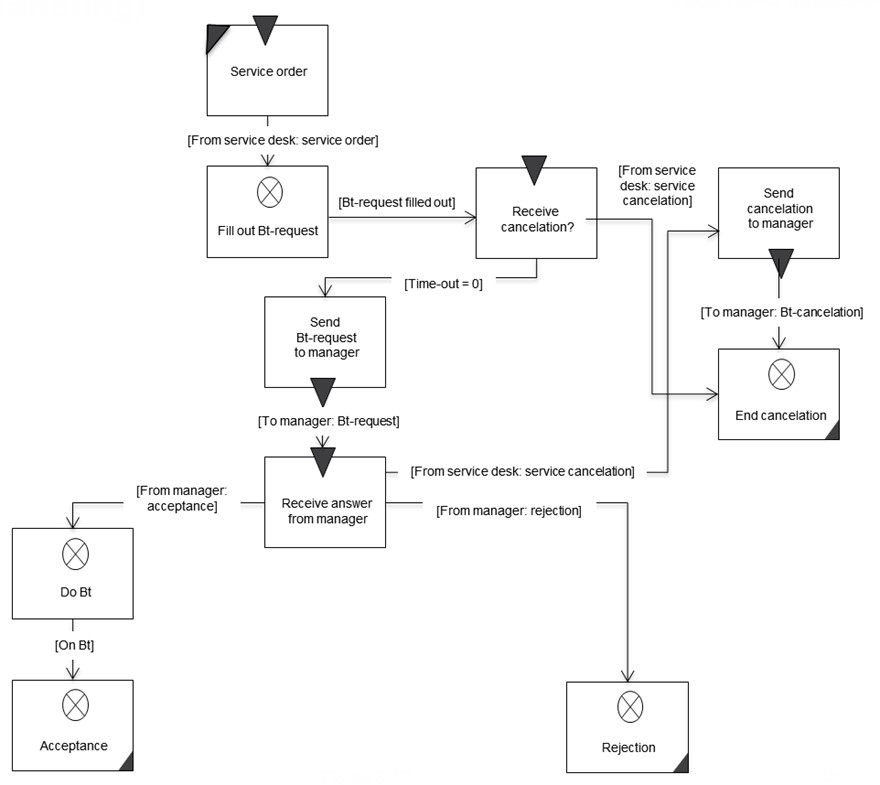
\includegraphics[width=0.7\linewidth]{20181026-Ontologie-Bilder/Grafiken-Ontologie/SUbjectExecution/ExceptionHandling}
	\caption[Handling the cancelation message using existing constructs]{Handling the cancelation message using existing constructs}
	\label{fig:exceptionhandling}
\end{figure}

A corresponding adjustment of the behavior must be made for each subject which can receive a cancellation message, including the manager, the travel office, and the interface subject 'travel agent'.

This relatively simple example already shows that taking such exception messages into account can quickly make behavior descriptions confusing to understand. The concept of exception handling, therefore, should enable supplementing exceptions to the default behavior of subjects in a structured and compact form. 

\begin{figure}[htbp]
	\centering
	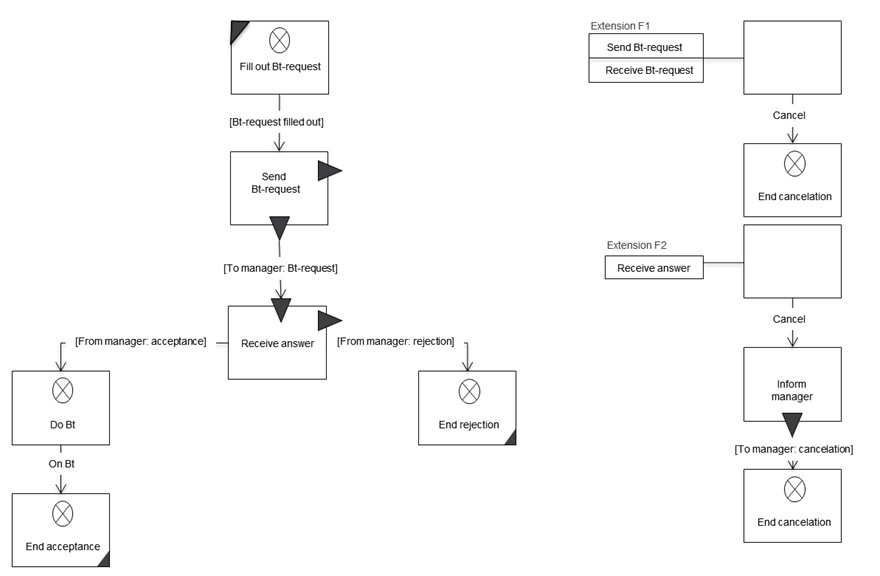
\includegraphics[width=0.7\linewidth]{20181026-Ontologie-Bilder/Grafiken-Ontologie/SUbjectExecution/Extension}
	\caption[Behavior of subject 'employee' with exception handling]{Behavior of subject 'employee' with exception handling}
	\label{fig:extension}
\end{figure}

Instead of, as shown in Figure \ref{fig:exceptionhandling}, modeling receive states with a timeout zero and corresponding state transitions, the behavioral description is enriched with the exception handling 'service cancellation'. Its initial state is labeled with the states from which it is branched to, once the message 'service cancellation' is received. In the example, these are the states 'fill out Bt-request' and 'receive answer from manager'. Each of them is marked by a triangle on the right edge of the state symbol. The exception behavior leads to an exit of the subject after the message 'service cancellation' has been sent to the subject 'manager'.

A subject behavior does not necessarily have to be brought to an end by an exception handling; it can also return from there to the specified default behavior. Exception handling behavior in a subject may vary, depending on from which state or what type of message (cancellation, temporary stopping of the process, etc.) it is called. The initial state of exception handling can be a receive state or a function state.

Messages, like 'service cancellation', that lead to exception handling always have higher priority than other messages. This is how modelers express that specific messages are read in a preferred way. For instance, when the approval message from the manager is received in the input pool of the employee, and shortly thereafter the cancellation message, the latter is read first. This leads to the corresponding abort consequences.

Since now additional messages can be exchanged between subjects, it may be necessary to adjust the corresponding conditions for the input-pool structure. In particular, the input-pool conditions should allow storing an interrupt message in the input pool. To meet organizational dynamics, exception handling and extensions are required. They allow taking not only discrepancies but also new patterns of behavior, into account.

\textbf{Behavior Extensions}---
When exceptions occur, currently running operations are interrupted. This can lead to inconsistencies in the processing of business objects. For example, the completion of the business trip form is interrupted once a cancelation message is received, and the business trip application is only partially completed. Such consequences are considered acceptable, due to the urgency of cancelation messages. In less urgent cases, the modeler would like to extend the behavior of subjects in a similar way, however, without causing inconsistencies. This can be achieved by using a notation analogous to exception handling. Instead of denoting the corresponding diagram with 'exception', it is labeled with 'extension'.

Behavior extensions enrich a subject's behavior with behavior sequences that can be reached from several states equivocally.

For example, the employee may be able to decide on his own that the business trip is no longer required and withdraw his trip request. Figure \ref{fig:extension} shows that the employee can cancel a business trip request in the states 'send business trip request to manager' and 'receive answer from manager'. If the transition 'withdraw business trip request' is executed in the state 'send business trip request to manager', then the extension 'F1' is activated. It leads merely to canceling of the application. Since the manager has not yet received a request, he does not need to be informed.

In case the employee decides to withdraw the business trip request in the state 'receive answer from manager', then extension 'F2' is activated. Here, first the supervisor is informed, and then the business trip is canceled.

\begin{figure}[htbp]
	\centering
	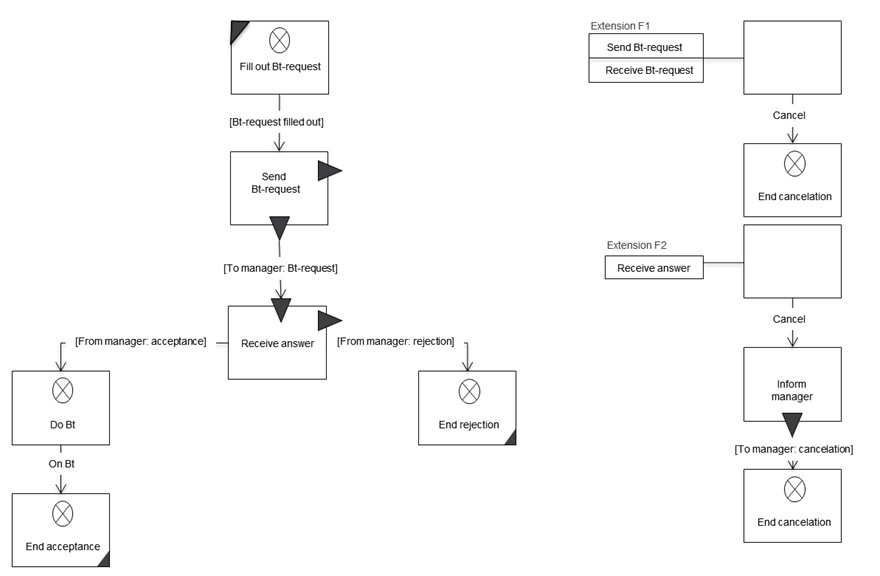
\includegraphics[width=0.7\linewidth]{20181026-Ontologie-Bilder/Grafiken-Ontologie/SUbjectExecution/Extension}
	\caption[Subject behavior of employee with behavior extensions]{Subject behavior of employee with behavior extensions}
	\label{fig:extension}
\end{figure}

\subsubsection{Alternative Actions (Freedom of Choice)} 

So far, the behavior of subjects has been regarded as a distinct sequence of internal functions, send and receive activities. In many cases, however, the sequence of internal execution is not important.

Certain sequences of actions can be executed overlapping. We are talking about freedom of choice when accomplishing tasks. In this case, the modeler does not specify a strict sequence of activities. Rather, a subject (or concrete entity assigned to a subject) will organize to a particular extent its own behavior at runtime.

The freedom of choice with respect to behavior is described as a set of alternative clauses which outline several parallel paths. At the beginning and end of each alternative, switches are used: A switch set at the beginning means that this alternative path is mandatory to get started, a switch set at the end means that this alternative path must be completely traversed. This leads to the following constellations:

\begin{itemize}
	\item Beginning is set/end is set: Alternative needs to be processed to the end.
	\item Beginning is set/end is open: Alternative must be started but does not need to be finished. 
	\item Beginning is open/end is set: Alternative may be processed, but if so must be completed.
	\item Beginning is open/end is open: Alternative may be processed but does not have to be completed.
\end{itemize}

The execution of an alternative clause is considered complete when all alternative sequences, which were begun and had to be completed, have been entirely processed and have reached the end operator of the alternative clause.

Transitions between the alternative paths of an alternative clause are not allowed. An alternate sequence starts in its start point and ends entirely within its endpoint.

Figure \ref{fig:alternative} shows an example for modeling alternative clauses. After receiving an order from the customer, three alternative behavioral sequences can be started, whereby the leftmost sequence, with the internal function 'update order' and sending the message 'deliver order' to the subject 'warehouse', must be started in any case. This is determined by the 'X' in the symbol for the start of the alternative sequences (the gray bar is the starting point for alternatives). This sequence must be processed through to the end of the alternative because it is also marked in the end symbol of this alternative with an 'X' (gray bar as the endpoint of the alternative).

\begin{figure}[htbp]
	\centering
	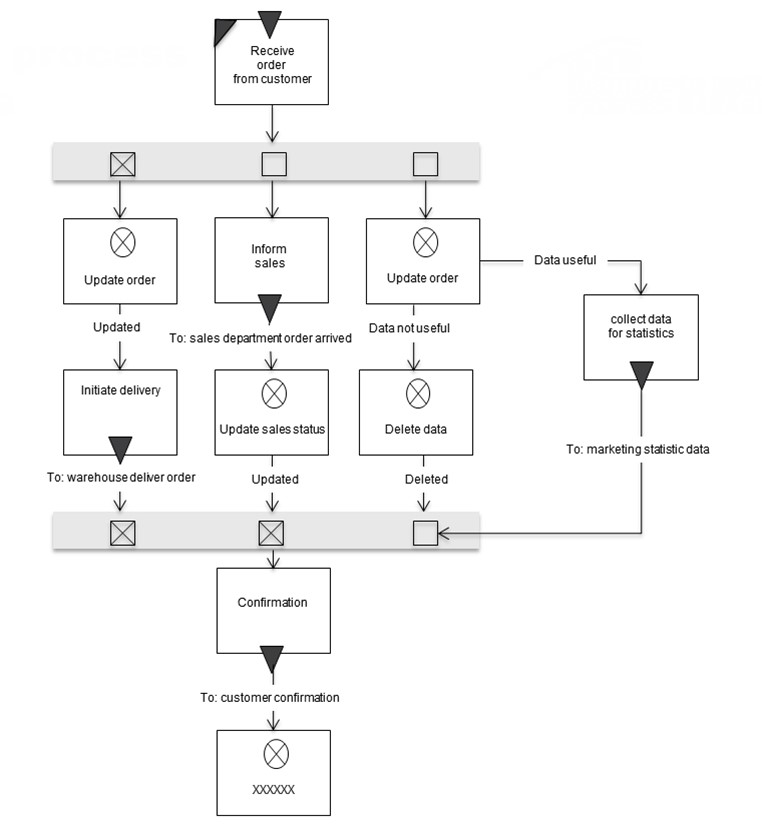
\includegraphics[width=0.7\linewidth]{20181026-Ontologie-Bilder/Grafiken-Ontologie/SUbjectExecution/ALternative}
	\caption[Example of Process Alternatives]{Example of Process Alternatives}
	\label{fig:alternative}
\end{figure}

The other two sequences may, but do not have to be, started. However, in case the middle sequence is started, i.e., the message 'order arrived' is sent to the sales department, it must be processed to the end. This is defined by an appropriate marking in the end symbol of the alternatives ('X' in the lower gray bar as the endpoint of the alternatives). The rightmost path can be started but does not need to be completed.

The individual actions in the alternative paths of an alternative clause may be arbitrarily executed in parallel and overlapping, or in other words: A step can be executed in an alternative sequence, and then be followed by an action in any other sequence. This gives the performer of a subject the appropriate freedom of choice while executing his actions.

In the example, the order can thus first be updated, and then the message 'order arrived' sent to sales. Now, either the message 'deliver order' can be sent to the warehouse or one of the internal functions, 'update sales status' or 'collect data for statistics', can be executed.

The left alternative must be executed completely, and the middle alternative must also have been completed, if the first action ('inform sales' in the example) is executed. Only the left alternative can be processed because the middle one was never started. Alternatively, the sequence in the middle may have already reached its endpoint, while the left is not yet complete. In this case, the process waits until the left one has reached its endpoint. Only then will the state 'confirmation' be reached in the alternative clause. The right branch neither needs to be started, nor to be completed. It is therefore irrelevant for the completion of the alternative construct.

The leeway for freedom of choice with regards to actions and decisions associated with work activities can be represented through modeling the various alternatives—situations can thus be modeled according to actual regularities and preferences.

\section{Ontology of Subject Behavior Description}

Each subject has a base behavior (see property 202 in \ref{fig:20190104-simple-elements-and-modellelement}) and may have additional subject behaviors (see class \texttt{SubjectBehavior} in \ref{fig:20190104-simple-elements-and-modellelement}) for macros and guards. All these behaviors are subclasses of the class \texttt{SubjectBehavior}. The details of these behaviors are defined as state transition diagrams (PASS behavior diagrams). These behavior diagrams are represented in the ontology with the class \texttt{BehaviorDescribingComponent} (see figure \ref{fig:20190104-simple-elements-and-modellelement}). The behavior diagrams have the relation \texttt{belongsTo} to the class \texttt{SubjectBehavior}. The other classes are needed for \texttt{embeddingsubjects} into the subject interaction diagram (SID) of a PASS specification (see chapter \ref{OWL-DescriptionSID}).

\begin{figure}[htbp]
	\centering
	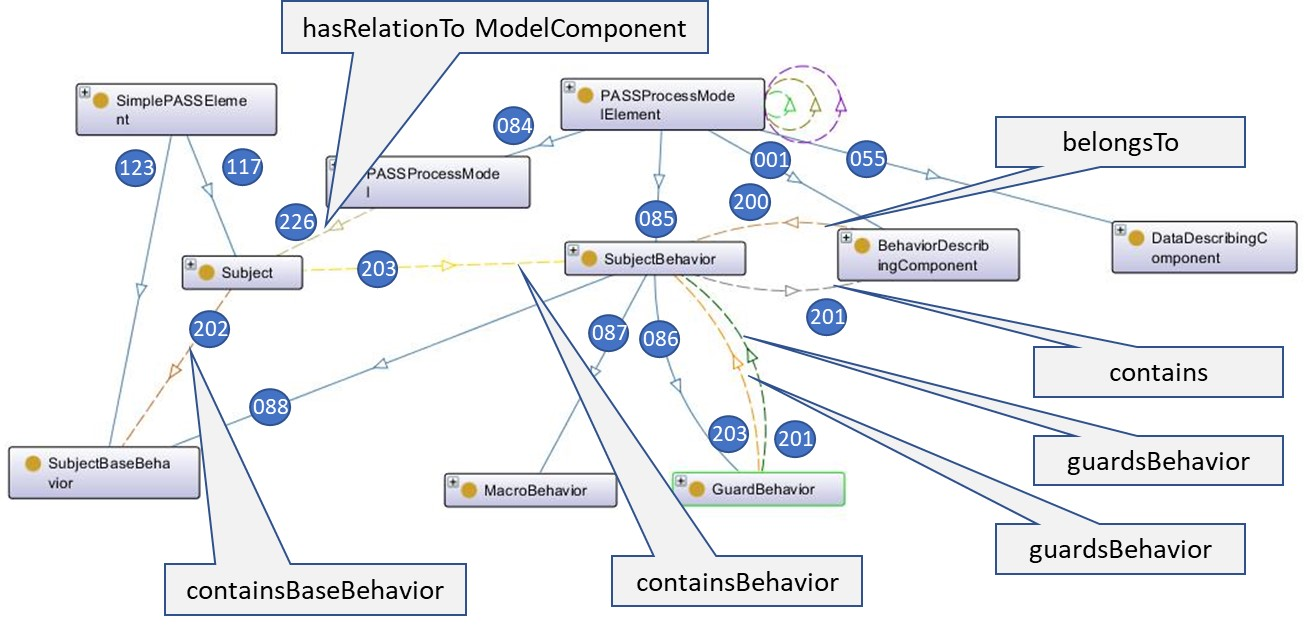
\includegraphics[width=0.9\linewidth]{20181026-Ontologie-Bilder/Grafiken-Ontologie/SUbjectExecution/20190104-SImple-Elements-and-Modellelement}
	\caption[Structure of Subject Behavior Specification]{Structure of Subject Behavior Specification}
	\label{fig:20190104-simple-elements-and-modellelement}
\end{figure}

\subsection{Behavior Describing Component}

The following figure shows the details of the class \texttt{BehaviorDescribingComponent}. This class has the subclasses State, Transition and \texttt{TranssitionCondition} (see figure \ref{fig:20190104-behavior-describing-component}). The subclasses of the state represent the various types of states (class relations 025, 014 und 024 in \ref{fig:20190104-behavior-describing-component}). The standard states \texttt{DoSTates}, \texttt{SendState} and \texttt{ReceiveState} are subclasses of the class \texttt{StandardPASSState} (class relations 114, 115 und 116 in \ref{fig:20190104-behavior-describing-component}). The subclass relations 104 and 020 allow that there exist a start state (class \texttt{InitialStatOfBehavior} in \ref{fig:20190104-behavior-describing-component}) and none or several end states (see subclass relation 020 in figure\ref{fig:20190104-behavior-describing-component}) The fact that there must be at least one start state and none or several end states is defined by so called axioms which are not shown in figure \ref{fig:20190104-behavior-describing-component}.

\begin{figure}[htbp]
	\centering
	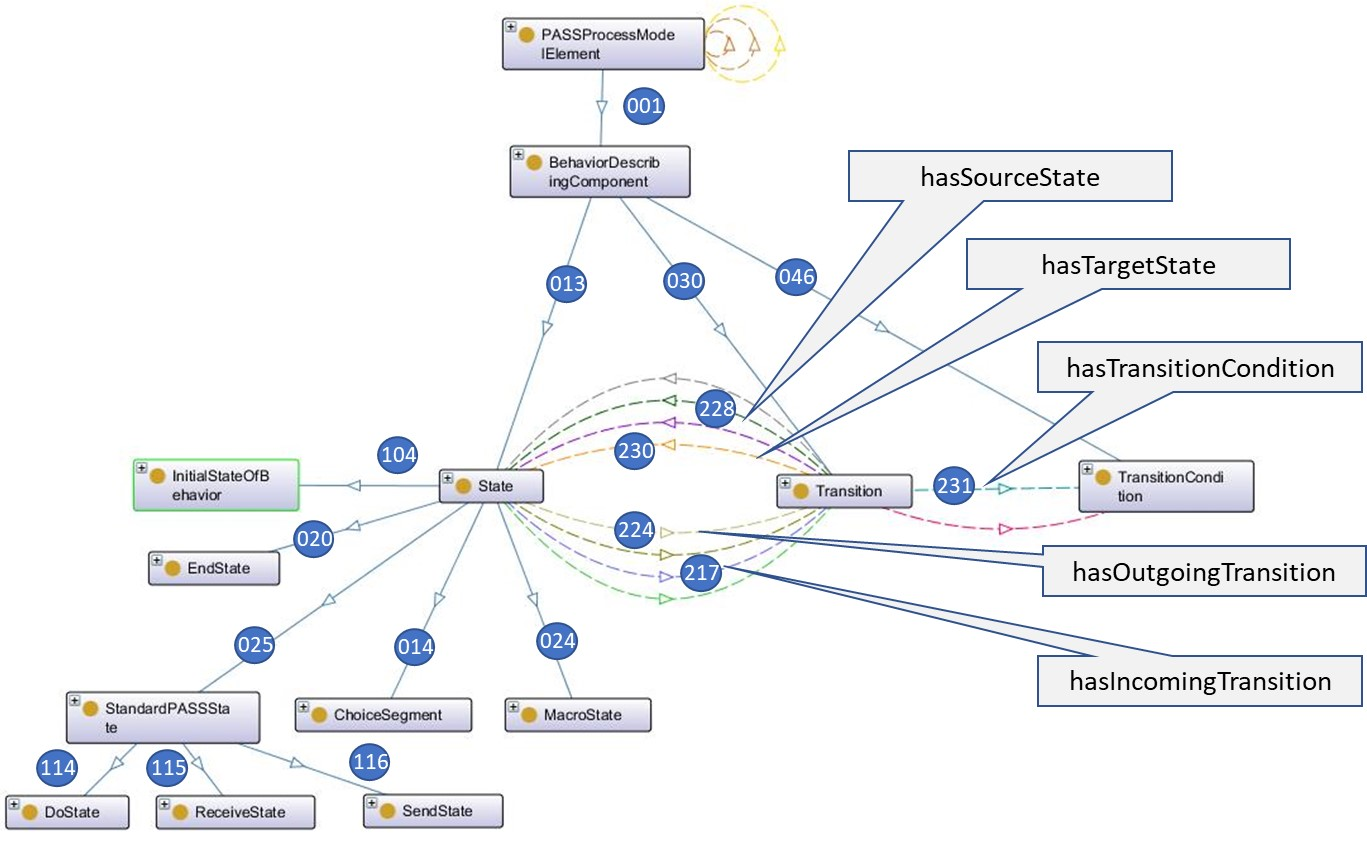
\includegraphics[width=1.0\linewidth]{20181026-Ontologie-Bilder/Grafiken-Ontologie/SUbjectExecution/20190104-Behavior-describing-component}
	\caption[Subject Behavior describingComponent]{Subject Behavior describingComponent}
	\label{fig:20190104-behavior-describing-component}
\end{figure}

States can be starting and/or endpoints of transitions (see properties 228 and 230 in figure \ref{fig:20190104-behavior-describing-component}). This means a state may have outgoing and/or incoming transitions (see properties 224 and 217 in figure \ref{fig:20190104-behavior-describing-component}). Each transition is controlled by a transition condition which must be true before a behavior follows a transition from the source state to the target state.

\subsubsection{States}

As shown in figure \ref{fig:20190109-states} the class state has a subclass \texttt{StandardPASSState} (subclass relation 025) which have the subclasses \texttt{ReceiveState}, \texttt{SendState} and \texttt{DoState}(subclass relations 027, 026, 025). A state can be a start state (subclass \texttt{InitialStateOfBehavior} subclass relation 022). Besides these standard states there are macro states (subclass 024). Macro states contain a reference (subclass 029) to the corresponding macro (Property 201).

\begin{figure}[htbp]
	\centering
	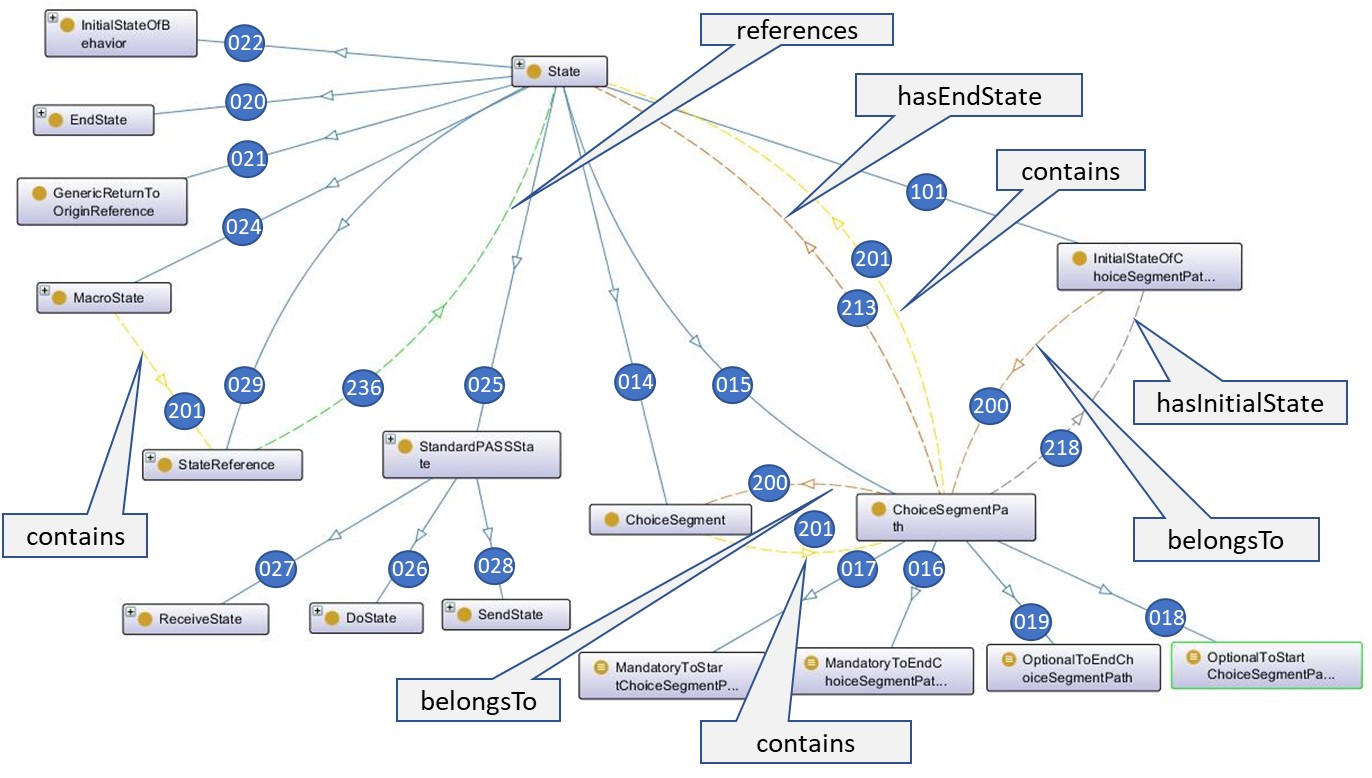
\includegraphics[width=1.0\linewidth]{20181026-Ontologie-Bilder/Grafiken-Ontologie/SUbjectExecution/20190109-States}
	\caption[Details of States]{Details of States}
	\label{fig:20190109-states}
\end{figure}

More complex states are choice segments (subclass relation 014). A choice segment contains choice segment paths (subclass 015 and property 200). Each choice segment path can be of one of four types. If a segment path is started than it must be finished or not or a segment path must be started and must be finished or not (subclass relations 16, 17, 18 and 19).

\subsubsection{Transitions}

Transitions connect the source state with the target state (see figure \ref{fig:20190104-behavior-describing-component}). A transition can be executed if the transition condition is valid. This means the state of a behavior changes from the current state which is the source state to the target state. In PASS there are two basic types of transitions, \texttt{DoTransitions} and \texttt{CommunicationTranstions} (subclasses 34 and 31 in figure \ref{fig:20190105-transitions}). The class \texttt{CommunicationTransition} is divided into the subclasses \texttt{ReceiveTransition} and \texttt{SendTransition} (subclasses 32 and 33 in figure \ref{fig:20190105-transitions}). Each transition has depending from its type a corresponding transition condition (property 231 in figure  \ref{fig:20190105-transitions}) which defines a data condition which must be valid in in order to execute a transition.

\begin{figure}[htbp]
	\centering
	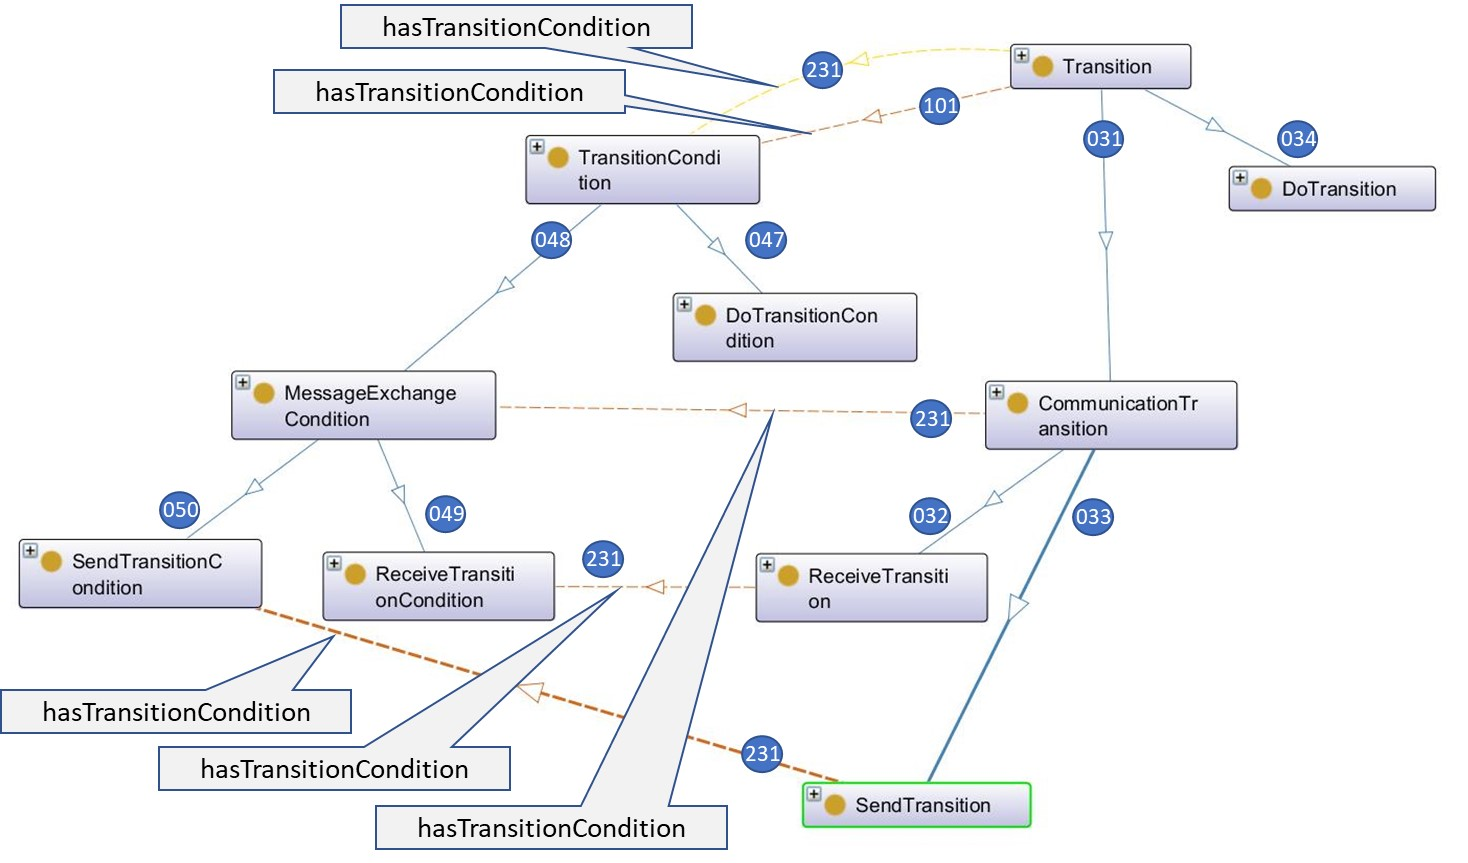
\includegraphics[width=1.0\linewidth]{20181026-Ontologie-Bilder/Grafiken-Ontologie/SUbjectExecution/20190105-Transitions}
	\caption[Details of transitions]{Details of transitions}
	\label{fig:20190105-transitions}
\end{figure}

\section{ASM Definition of Subject Execution}

\texttt{Behavior(subj;state)} is the ASM-Rule to interpret a specific node of a behavior diagram for a specific subject.

It expresses that when a subject in a given state has completed a given action (function, send or receive operation)---read: Performing the action has been completed while the subject was in the given SID-state. Assuming that the action has been started by the subject upon entering this state-then the subject proceeds to start its next action in its successor state. The successor state is determined by an \texttt{ExitCondition} whose value is defined by the just-completed action. Figure \ref{fig:asm-behavior} shows the ASM code for the behavior rule.

\begin{figure}[htbp]
	\centering
	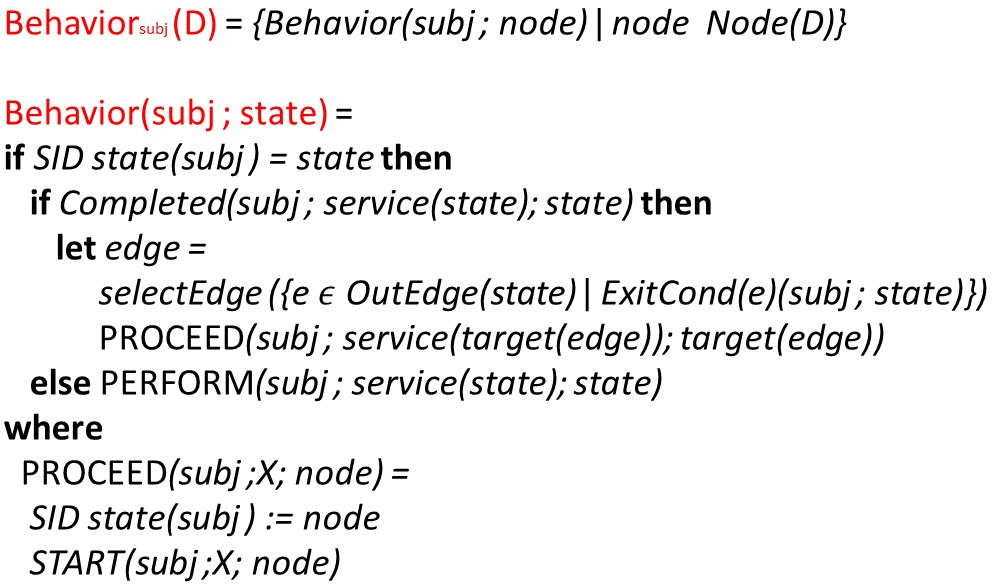
\includegraphics[width=0.7\linewidth]{20181026-Ontologie-Bilder/Grafiken-Ontologie/SUbjectExecution/ASM-Behavior}
	\caption[ASM Code for Behavior]{ASM Code for Behavior}
	\label{fig:asm-behavior}
\end{figure}

The complete ASM based definition of PASS was developed by Egon Börger and can be found in Annex \ref{ASM-Interpreter}.

\subsection{Internal Functions/Action}

A detailed internal \texttt{Behavior} of a subject in a state with internal function A can be defined in terms of the ASM sub-machines \texttt{Start} and \texttt{Perform} together with the predicate \texttt{Completed} for the parameters \texttt{(subj ;A; state)} in the same manner as has been done for communication actions in section \ref{CommunicationAction} but only once it is known how to start, to perform and to complete A. For example, \texttt{Start(subj ;A; state)} could mean to call function A which is implemented as a method of a class. The completion predicate coincides with the termination condition of the method. 

\subsection{Communication Action}
\label{CommunicationAction}

\begin{figure}[htbp]
	\centering
	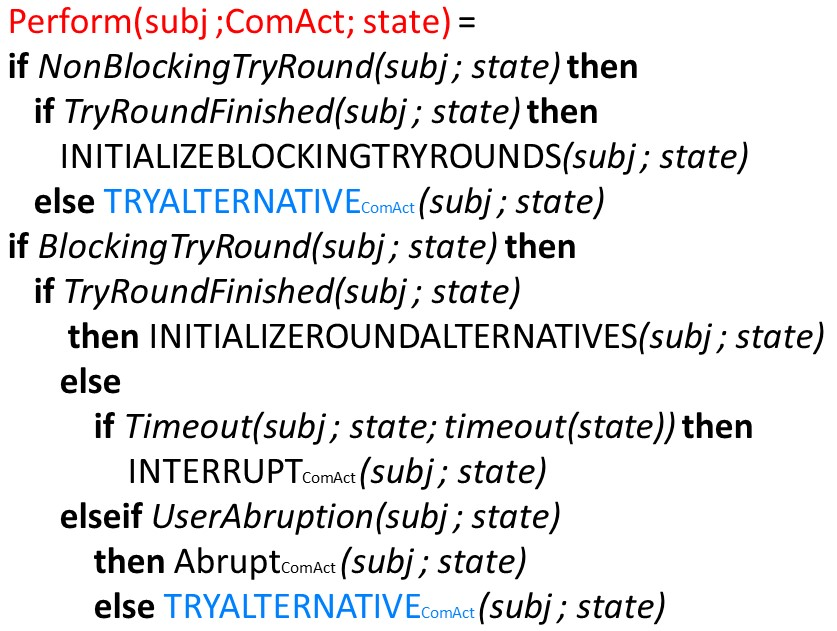
\includegraphics[width=0.7\linewidth]{20181026-Ontologie-Bilder/Grafiken-Ontologie/SUbjectExecution/ASM-perform}
	\caption{}
	\label{fig:asm-perform}
\end{figure}


\backmatter
% bibliography, glossary and index would go here.

\end{document}